\chapter{O impacto da evolução da óptica na arte --- lente, câmera e projetor}%
\label{cap2-impacto-evolucao-otica}

Neste capítulo abordamos dois assuntos que se relacionam com o tema
principal de nosso estudo: a evolução da óptica e o que caracteriza o
olhar do cinema, sob uma perspectiva de ordem prática. Para isto,
revisitamos textos de alguns autores que se colocam nesta intersecção.

Durante o período de estudos na Escola de Artes Visuais, chamou-me a
atenção um livro da bibliografia, que então servia de base para um dos
cursos, intitulado \citetitleyear{flores2011fotografia}. Como
temos observado, pintores contemporâneos passaram a se utilizar de
fotografias como modelo para suas obras. Em seu texto, \textcite{flores2011fotografia}
reflete sobre as características das duas disciplinas, com a hipótese de que
\enquote{Fotografia e Pintura são, no fundo, a mesma coisa}
\parencite[7]{flores2011fotografia}. Não estamos tratando aqui do mesmo
paradigma da autora, que trata da Fotografia e Pintura nos termos de
serem iguais ou diferentes, e de como, se conectam estes dois campos
presentes na vida diária, com os quais se lida de maneira diferente.
Nosso objetivo é investigar a possibilidade de se usar o olhar
característico do cinema na construção de uma pintura. Como ponto de
partida nos parece adequado lembrar o crítico e teórico do cinema,
André Bazin, que realiza uma \emph{ponte} entre pintura, fotografia e
cinema, através de seu texto \citetitleyear{bazin1983ontologia}.
Trazemos para este capitulo um apontamento de um dos primeiros ensaios
de \textcite{bazin1983ontologia}, que é um estudo retomado a partir de
\emph{Problèmes de la Peinture}\footnote{\enquote{Problemas de pintura}
	--- tradução nossa}, 1945.

\begin{displaycquote}[125]{bazin1983ontologia}[.]
	A originalidade da fotografia em relação à pintura reside, pois, na sua
	objetividade essencial. Tanto é que o conjunto de lentes que constitui o
	olho fotográfico em substituição ao olho humano, denomina-se
	precisamente \emph{objetiva}. Pela primeira vez, entre o objeto inicial
	e sua representação nada se impõe, a não ser um outro objeto. Pela
	primeira vez, uma imagem do mundo exterior se forma, automaticamente,
	sem a intervenção criadora do homem, segundo um rigoroso determinismo. A
	personalidade do fotógrafo entra em jogo somente pela escolha, pela
	orientação, pela pedagogia do fenômeno; por mais visível que seja na
	obra acabada, já não figura nela como a do pintor
\end{displaycquote}

O aspecto de que fotógrafo e pintor deixam a marca de sua personalidade
de forma diferente em suas obras, pode ser questionado diante da cena
contemporânea, na medida que ambos realizam escolhas cujo objetivo é se
expressar por meio de seus projetos. Os instrumentos podem ser
diferentes, mas os objetivos nos parecem comuns e o problema da escolha
do processo que cada artista adota para tratar de seu assunto ou tema,
muito nos interessa nesta investigaçāo, que estará será aprofundado no
\cref{cap3-narrativa-visual}.

Por hora, queremos destacar neste texto o ponto que diz haver pela
primeira vez um dispositivo que passou a intermediar o método de
criação, tanto da fotografia quanto do cinema. A câmera e suas lentes
evoluem a partir do que Bazin caracteriza ser um acontecimento
decisivo:

\begin{displaycquote}[125]{bazin1983ontologia}[.]
	\textelp{} a invenção do primeiro sistema científico e, de certo modo, já
	mecânico: a perspectiva (a câmara escura de Da Vinci prefigurava a de
	Niepce). Ele permitia ao artista dar a ilusão de um espaço de três
	dimensões onde os objetos se podiam situar como na nossa percepção
	direta
\end{displaycquote}

Para ele, diferente da pintura, a fotografia e o cinema tinham uma
mesma origem, a mecânica, e entre o objeto inicial e sua representação
não havia a intervenção humana. Neste sentido, Bazin demonstra confiar
na imparcialidade do aparato técnico da câmera.

Um outro ponto de vista é abordadado por Comolli (1941--2022), nos
ensaios sobre a teoria e história do cinema, publicados nos Cahiers du
Cinema (1971), onde agrega a herança ideológica da câmera à sua herança
científica. Para \textcite{comolli2015cinema} o que está em causa é estatuto técnico
de invisibilidade da câmera na produção do espetáculo e os
investimentos ideológicos tanto na produção do filme quanto em uma
teoria criada com fins políticos \parencite{comolli2015cinema}.

Com relação a esta discussão, \textcite{grilo1993ordem}
observa que \enquote{o termo objectiva talvez seja então um termo pelo
	menos equívoco para designar o sistema óptico utilizado nas câmaras
	fotográficas, de cinema e televisão}. Para ele a contribuição de
Comolli foi importante na época para enfatizar a \enquote{natureza
	arbitrária dos códigos de representação incorporados na tecnologia
	básica do cinema} \textelp{} \emph{ficção geométrica} que impõe ao real
(com o qual se assemelha) uma \emph{rectificação ideológica}
\parencite[332-333]{grilo1993ordem}.

\begin{displaycquote}[331-332]{grilo1993ordem}[.]
	Comoli e Pleynet promovem uma crítica poderosa aos princípios bazinianos
	de Ontologia da Imagem Cinematográfica, problematizando o caráter
	automático da representação fílmica e desconstruindo a pregnância do
	óptico sobre o ideoláqico. \textelp{} A imagem do cinema é, enquanto imagem
	perspéctica, uma imagem organizada \textelp{} atribui a este olho e, portanto
	ao sujeito que olha --- pela coincidência geométrica entre o ponto de
	vista~e o ponto de fuga --- um lugar privilegiado e central
\end{displaycquote}

\section{Óptica e movimento na pintura }%
\label{sec:optica-e-movimento-na-pintura}

\paragraph{Sobre a óptica} O conhecimento secreto dos pintores renascentistas, descrito na
publicação do pintor David Hockney (1937), \emph{Secret Knowledge:
	Rediscovering the Lost Techniques of the Old
	Masters}\footnote{\enquote{Conhecimento Secreto: Redescobrindo as
		Técnicas Perdidas dos Antigos Mestres} --- tradução nossa.} (2001), e
divulgado através do documentário de TV produzido pela BBC,
\hiperlink{https://www.imdb.com/title/tt0387965/?ref\_=ttpl\_pl\_tt}{\emph{David
		Hockney: Secret Knowledge}} (2002)\footnote{Documentário \emph{David
		Hockney Secret Knowledge}
	\url{http://www.youtube.com/watch?v=JKbFZIpNK10\&t=14s\&ab_channel=taylordiabennett}}
relata as técnicas dos mestres da idade clássica da pintura, e sobre
como são vistas e tratadas as imagens hoje, na era da manipulação
digital. O autor apresenta seu estudo teórico sobre como algumas das
famosas obras-primas da arte ocidental de artistas como Da Vinci,
Caravaggio, Velazquez e Van Eyck foram realmente criadas. Segundo
Hockney, o espelho e as lentes já eram usados como técnicas de
reprodução da imagem, que se desdobraram na fotografia atual. O método
utilizado à época tinha por finalidade auxiliar na estruturação de suas
pinturas. A matemática teve então um novo aliado: as descobertas da
física e da óptica que traziam o novo dispositivo técnico ao serviço da
pintura, se propagando entre os pintores do século XIX. Portanto, a
arte bidimensional já tinha uma afinidade grande com o que se chamaria
de fotografia, antes mesmo dos \enquote{primeiros filmes}.

O uso de projetores para iniciar um trabalho pictórico, processo comum
a muitos pintores contemporâneos, vem se somar aos tradicionais esboços
com os modelos vivos e técnicas de ampliação de desenho. Abordaremos
este assunto mais adiante, no \cref{cap4-entre-projeto-processo}, ao tratar de um método
fundamental utilizado em nosso processo de pintura.

\paragraph{Sobre o movimento} O desejo humano de reproduzir o movimento, se manifesta na imagem
pictórica e na imagem fílmica através do direcionamento do olhar.
Buscamos aqui respostas à inquietação que temos em saber como nossos
olhos se movimentam diante de uma pintura, quando guiados pela
composição. O conceito de movimento, para além de ser uma metáfora do
primeiro tema das pinturas deste mestrado em artes plásticas, que eram
as malas, possuía relevância como objeto de pesquisa relacionado ao
direcionamento do olhar, um assunto que me interessava tanto na pintura
quanto no cinema. O início de nossa pesquisa se ancorou na palavra
movimento, que se apresenta sempre que associamos imagens de figuras
estáticas representadas na pintura às do cinema:
\enquote{\emph{impressão de movimento}}. Como veremos adiante, os
estudos de representação do movimento, identificados em Leonardo Da
Vinci e Rubens, complementaram o nosso entendimento sobre o escopo
deste texto, que se ancora na visualidade.

\paragraph{A forma do filme e o sentido da pintura}
As teorias da visualização iniciadas com a invenção da perspectiva em
Florença, entre 1420 e 1450, atribuída ao arquiteto Bruneleschi
\parencite{arasse2016historias}, têm um encontro marcado com o cinema nos experimentos
do psicólogo Rudolf Arnheim, com sua psicologia da forma
(\emph{Gestalt}). Arnheim teoriza sobre o filme no livro \emph{Film as
	Art} (1932), antes mesmo de escrever sua principal obra \emph{Arte e
	Percepção Visual:~uma psicologia da visão criadora} (1954).
Estuda as relações espaciais no quadro e a percepção visual,
podendo ser considerado um marco do encontro da narrativa pictórica com
a do cinema. Seus estudos trouxeram um novo olhar para o ensino não só
dentro das academias, mas também para a pintura contemporânea. No
artigo \emph{Percepção e Estética na Teoria do Cinema de Hugo
	Münsterberg e de Rudolf Arnheim}, \citeauthor{pedro2013percepcao}~\cite*{pedro2013percepcao}
relaciona dois autores muito estudados nas escolas de cinema e de pintura, ao
demonstrar que a estética do cinema é fundamentada por uma teoria da
percepção em dois textos marcantes da teoria clássica do cinema, o
texto de Hugo Münsterberg (1916) e a obra de Rudolf Arnheim, \emph{Film
	as Art} (1932). \textcquote[226]{pedro2013percepcao}[.]{Neste sentido,
	estes dois textos oferecem um exemplo paradigmático para pensar a
	interseção entre teoria da percepção e estética}.

Encontramos na produção contemporânea da pintura figurativa, uma grande
utilização destas teorias em suas técnicas compositivas, muitas delas
relacionadas ao movimento do olhar percorrendo a tela na pintura. Não
podemos deixar de relacionar os conceitos perceptivos das diagonais de
Arnheim, seu estudo sobre peso, equilíbrio, e percepção no esqueleto
estrutural do quadrado, ao cruzamento do trem dos Lumière no ecrã, em
direção ao espectador. A direção do olhar tem sido explorada na arte
contemporânea, não só através de pinturas que tratam do assunto por
meio de apropriações, mas também quando a pintura fala da própria
pintura, em especial na pintura figurativa.

\begin{figure}
	\caption{\artname{Muntean \& Rosenblum}{Untitled (\enquote{To know anything\ldots})}{2020}}

	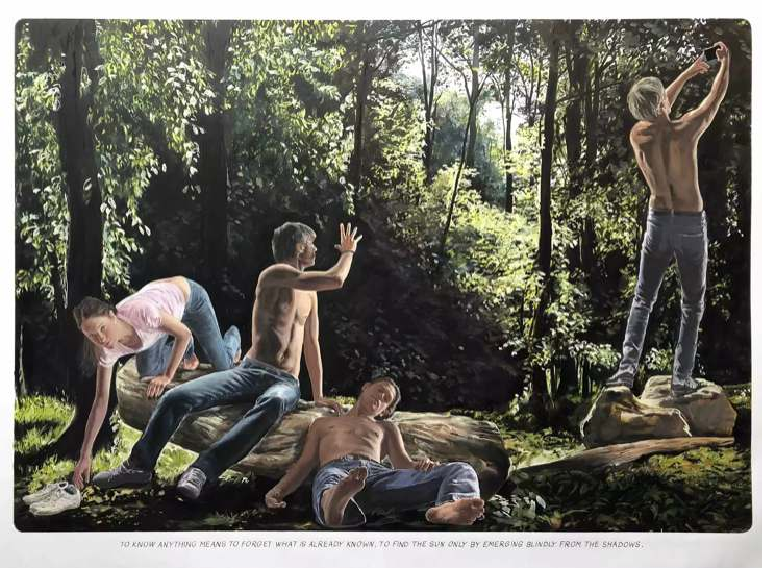
\includegraphics[width=4in,height=2.87832in]{figuras/muntean-rosenblum-to-know-anything-2010.pdf.compressed.pdf}
	\figurenote{Crayon, oil, acrylic on canvas. \artsize{225 x 305}. Fonte: \hiperlink{Artsy}{artsy.net/partner/galerie-ron-mandos}}
\end{figure}

Um exemplo disto é a dupla Muntean \& Rosenblum que traz a tradição da
pintura através da apropriação de estudos do espaço pictórico
realizados por autores como Alberti (1401--1472), Piero~Della Francesca
(1415--1492) e Lucca Pacioli (1445--1510). Segundo
\textcite[34]{sabino2000pintura}, \enquote{o pintor Piero Della~Francesca
  dedicou grande entusiasmo ao papel da matemática no
	entendimento da natureza, esmerando-se nos estudos sobre a
	geometrização do plano pictórico e a conquista da profundidade do
	espaço através da perspectiva.} Seu amigo Luca Pacioli que também se
relacionava na época com Alberti e Leonardo, era professor de
matemática e geometria em vários centros universitários da época como
Perugia, Urbino, Milão, Florença, Roma, Bolonha e Veneza. Sua obra
\emph{Da Divina Proporção} explica pela primeira vez a proporção de
ouro, com figuras geométricas regulares e sólidos tridimensionais. \parencite{sabino2000pintura}

Para \textcite{viveiros2007espacos}, a pintura holandesa e flamenga dos
séculos XVI e XVII constituíram um modelo alternativo à perspectiva da
pintura florentina do século XV. A imagem tornou-se num mapa amplo, mas
plano, onde o espectador se perdeu por não haver um centro de atração,
e sim um \emph{fluxo do olhar}. \parencite{viveiros2007espacos}

\begin{displaycquote}[38]{viveiros2007espacos}[.]
	A densidade visual da pintura flamenga e holandesa refletiu uma nova
	forma de conceber o mundo e o olhar, traduzido em amplas paisagens
	minuciosamente descritas e povoadas por diversas situações e
	acontecimentos, em mapas de lugares que nivelaram num efeito de
	superfície o próximo e o longínquo
\end{displaycquote}

Trazemos aqui um caso sobre a pintura flamenga que parte do cinema para
a pintura. O cineasta, pintor e diretor teatral polonês, Lech Janusz
Majewski realizou um tríptico fílmico, cuja principal peça \emph{O
	moinho e a Cruz} (2011) com roteiro de Gibson e Majewski utiliza
técnicas de CGI (\emph{computer-genereted imagery}) e efeitos em 3D
para realizar a transposição do livro \emph{Portement de Croix Historie
	d`um tableau de Pierre Bruegel l`Aîne} (1996), que analisa a pintura
\emph{Cristo carregando a cruz} (1564), de Pieter Bruegel, o Velho.

As estratégias de Bruegel e Majewski voltadas para a imersão do
espectador, em uma obra de arte, se utilizam de parâmetros
Renascentistas, como \emph{invenção} da paisagem, geometria euclidiana,
perspectiva \emph{artificialis} e cromática, e são analisadas no texto
de \textcite{lopes2019imersao}.

\begin{displayquote}{lopes2019imersao}[.]
	Estas descobertas, somadas a leituras, usos e conceitos de épocas
	subsequentes como sublime, \emph{contemplatio}, forma panorama, modelo
	panóptico, campo de mira x campo visual, perspectivas fisiológicas e
	múltiplas, apreendidas de forma sintética, serviram de base para a
	compreensão do processo de imersão do espectador numa obra de arte
\end{displayquote}

O maior desafio de Majewski para a reconstrução da pintura de Bruegel
no ecrã do cinema foi representar a perda da centralidade da
perspectiva \emph{artificialis},\footnote{Por ser baseado em leis
	matemáticas (científicas) de construção de espaço, a~\emph{perspectiva
		artificialis}~deveria dar a sensação mais parecida com a da visão por
	meio do olho humano, e criar assim a perspectiva mais próxima da imagem
	real.
	\url{https://andreamerico.wordpress.com/2011/03/29/a-geometria-de-alberti/}}
preponderante à época na Itália, que passou a se fracionar em sete ou
mais perspectivas difusas sobre a superfície plana. Por meio de
técnicas de~animação em 3D e computação eletrônica, montou o plano de
filmagem com o mesmo cruzamento~de linhas arquitetado por Bruegel.
Majewski usa o próprio personagem Bruegel (Hauer) em cena, traçando
diagonais e linhas perpendiculares e paralelas num papel. Esta
representação narrativa de Majewski vem ao encontro da sensação de
imersão que vivencio diante de cenas projetadas, tanto~na qualidade de
espectadora que reconstrói imagens mentais a partir de proposições
fílmicas, quanto na~condição de pintora, ao me posicionar entre o
projetor e a tela para recriar uma imagem já existente.

Se estamos tratando aqui de uma construção da imagem na pintura, pelo
olhar do cinema, cabe lembrar a motivação da perspectiva
\emph{artificialis} e anamorfose\footnote{Sobre anamorfose --- video
	do canal The Met --- \url{https://youtu.be/cEfwbnMf3jM}} no período
renascentista da pintura. Esta história está ligada ao desejo de
sistematizar a relação entre os olhos e a forma como eles veem, a fim
de representar a tridimensionalidade no plano bidimensional. Com o
avanço da representação alargada da paisagem, na pintura do século XV,
no Norte da Europa, surge um espaço amplo a ser percorrido pelo
espectador. Na pintura de Bruegel \emph{Cristo carregando a cruz},
conforme descreve \textcite{lopes2019imersao}:

\begin{displaycquote}[16]{lopes2019imersao}[.]
	O quadro pode ser lido também como um filme prestes a ser editado em
	fabulosas sequências por nós, seus interlocutores, numa linguagem cheia
	de ritmos, sons, luzes, cores e surpresas de combinações quase infinitas
	(\ldots) seguem um percurso mapeado da esquerda para a direita,
	perfazendo o próprio calvário de Jesus
\end{displaycquote}

Podemos estabelecer uma conexão do movimento do olhar, dentro do espaço
proposto pela pintura em Bruegel com a noção de imagem em movimento dos
primeiros filmes na década de 1890, e até mesmo antes, com a fotografia
\emph{The Horse in Motion} do galope de um cavalo quadro a quadro
realizada por Muybridge em 1878, usando uma série de 24 câmeras.

\begin{displaycquote}[25]{lopes2019imersao}[.]
	O que Bruegel fez, basicamente, foi a montagem de diferentes pontos de
	vista da forma como o olho humano trabalha no espaço. Portanto, é
	natural quando você olha para a tela. Você nem mesmo sente que ele está
	combinando diferentes perspectivas (Majewiski, depoimento, 2014)
\end{displaycquote}

O movimento ocular não é estático e se move diante da pintura de
Bruegel, provocando ilusões de profundidade. Remete à
\enquote{sensação} de movimento proposta pelo cinema. Estratégias que
querem dar veracidade à história contada e capturar o espectador para
dentro de um mundo que se pretende real. Segundo \textcite[24]{lopes2019imersao}
\enquote{Os movimentos inconscientes do olho não são apenas auxiliares
	que tornam a visão mais clara; são condições \emph{sine qua non} da
	visão. \textelp{} A visão estática não existe; não existe visão sem
	exploração (Koestler conforme citado em Crary, 2013, p.293).}

Segundo \textcite{focillon1983vida}, a obra de arte só é imóvel na
aparência: Ela exprime um desejo de imobilidade, é uma pausa, mas como
um momento no passado. Na realidade ela nasce de uma mudança e prepara
outra. Ele nos traz o exemplo de desenhos em que os mestres, superpõem
vários braços ligados ao mesmo ombro, na busca da perfeição. Os esboços
de Rembrandt estão presentes e vivem na pintura de Rembrandt. O esboço
dá movimento à obra prima \parencite[18]{focillon1983vida}.

Um movimento engendrado pela composição formal, em momentos extremados
como o da matemática e perspectiva com origem no período renascentista,
serve de base ao que Focillon chama de aparente imobilidade da obra de
arte, como mencionamos anteriormente. Na pintura \emph{O massacre dos
	inocentes}, de Rubens, o corpo do homem serve ao movimento das
simetrias, dos contrapostos e das alternâncias \parencite{focillon1983vida}.

\begin{figure}
	\caption{\artname{Rubens}{Massacre dos Inocentes}{1611/12}}
	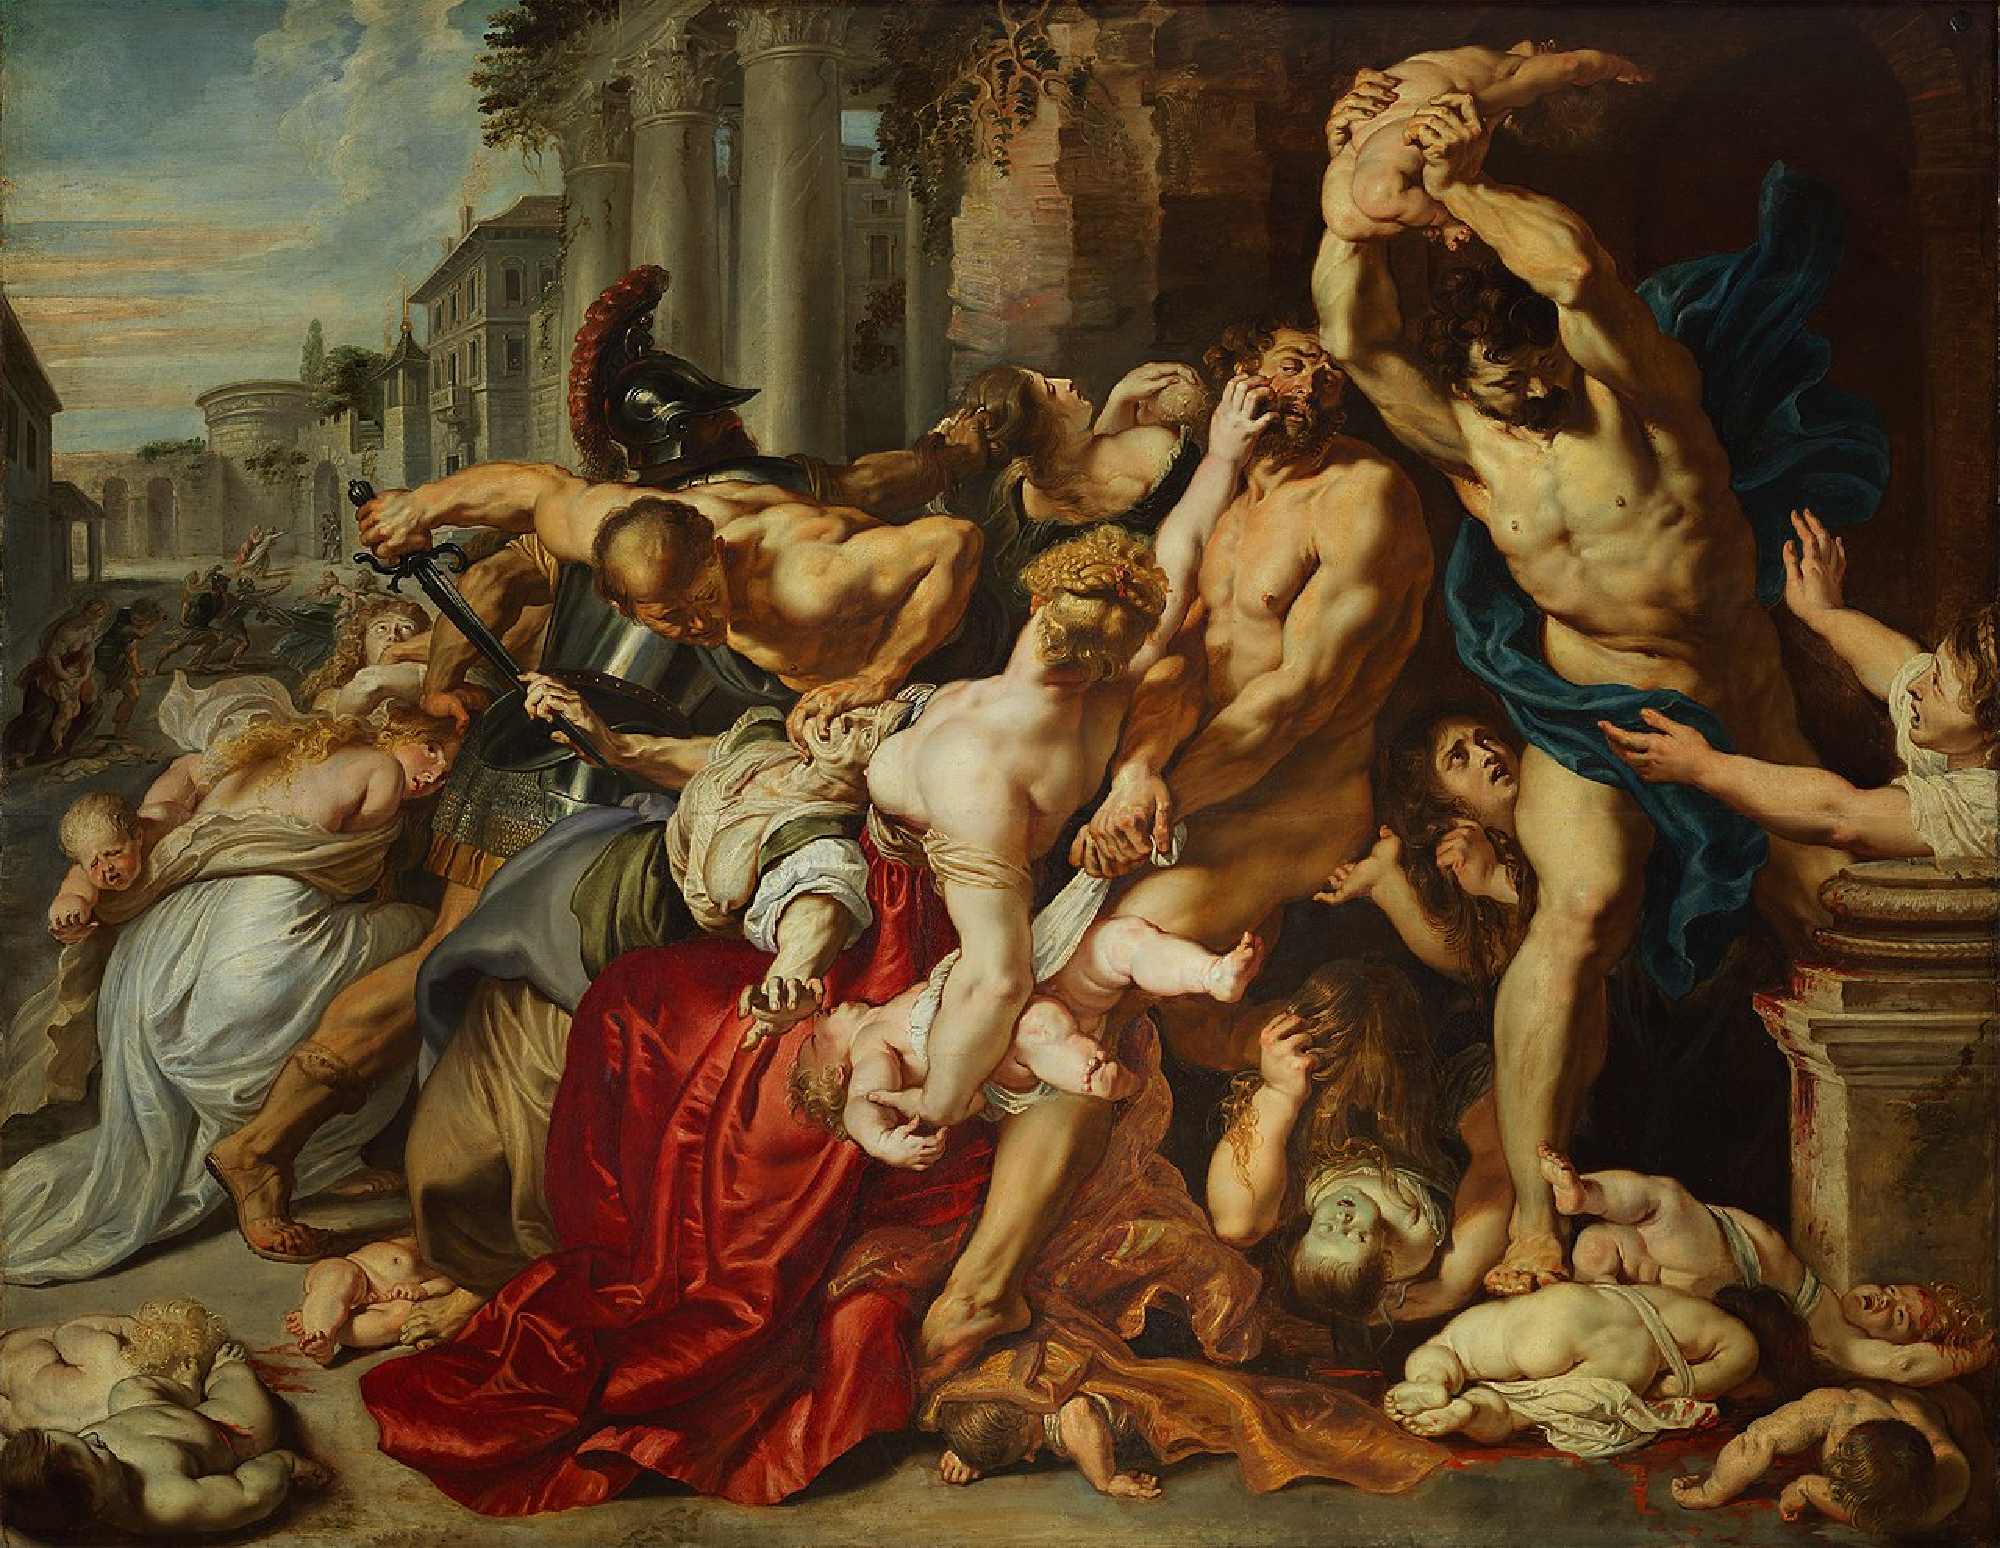
\includegraphics[width=3.88044in,height=3.00417in]{figuras/rubens-massacre-inocentes-1612.pdf.compressed.pdf}
	\figurenote{Galeria de arte de Ontário Fonte:
		\hiperlink{https://upload.wikimedia.org/wikipedia/commons/c/cf/Rubens_-_Massacre_of_the_Innocents_-_Art_Gallery_of_Ontario_2.jpg}{Wikimedia}}
\end{figure}

Neste sentido, \emph{La vie des formes} é sem dúvida um importante
trabalho a ser considerado na pesquisa sobre as relações entre o
movimento na pintura e no cinema. Embora a arte contemporânea tenha
superado a tendência formalista dos anos que precederam a segunda
guerra, cuja sistematização da história da arte é proposta na obra
\emph{Vida das Formas}, deve-se reconhecer a importância que os estudos
estéticos de Focillon proporcionaram e ainda encontram eco na prática e
no ensino das artes visuais.

A arte, com frequência, caminha para frente olhando para trás. Artistas
ao longo da história, viajaram através de países e continentes,
buscando se impregnar pelo olhar do outro. O interesse de Rubens pelos
estudos de Leonardo sobre movimento vem sendo aprofundado, no âmbito da
história da arte e curadoria, por
\textcite{barone2009rubens}. O texto
\emph{\citetitleyear{barone2009rubens}}, analisa as formas como Rubens
utilizou obras de Leonardo com foco no movimento.
\textcite{barone2009rubens} destaca:

\begin{displaycquote}[445]{barone2009rubens}[.]
	A importância para Rubens dos movimentos corporais em conexão com as
	atitudes mentais (que Leonardo considera a chave para a representação
	bem-sucedida do movimento) é corroborada em sua inscrição no canto
	superior direito do desenho Getty: \emph{'Gestus magis largi longi(que)
		bachijs extensis' (os} gestos \textins{serão} maiores e mais amplos, com os
	braços estendidos
\end{displaycquote}

Uma análise detalhada de dois desenhos de Rubens, quando confrontados
com \emph{A Última} Ceia de Leonardo (1495--1498), demonstra
similaridades claras entre gestos eloquentes e expressões fisionômicas
marcantes \parencite[443-444]{barone2009rubens}.


\begin{figure}
\begin{minipage}[b]{3.21905in}
	\caption[\artname{Leonard Da Vinci}{A última ceia}{1495--1498}]{\artname{Leonard Da Vinci}{A última ceia}{1495--1498}\footnotemark}
	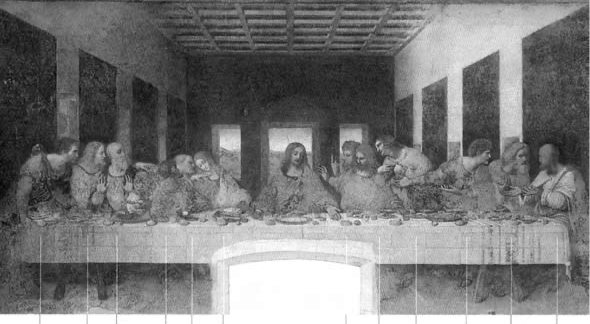
\includegraphics[width=3.21905in]{figuras/leonardo-ultima-ceia-1498.pdf}
	\figurenote{Fonte: \textcite{barone2009rubens}}
\end{minipage}\hfill
\begin{minipage}[t]{2.69403in}
	\caption{\artname{Peter Paul Rubens}{Grupos de apóstolos na última ceia}{1601--1604}}
	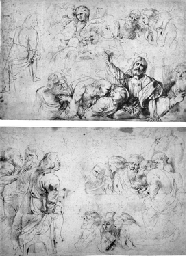
\includegraphics[width=2.39403in]{figuras/rubens-desenhos-selecionados-1986.pdf}
	\figurenote{Chatsworth (figura superior), Getty Museum (figura inferior).
		Fonte: \textcite{barone2009rubens}}
\end{minipage}
\end{figure}

\footnotetext{Na Última
	Ceia de Leonardo, da direita para a esquerda, os personagens são:
	Simão, Tadeu, Mateus, Filipe, Tiago Maior, Tomé, Cristo, João, Pedro,
	Judas, André, Tiago Menor e Bartolomeu.}

No próximo subitem objetivamos conceituar o que seria o olhar do cinema
a partir da definiçāo de termos utilizados pelo setor audiovisual, e
também através das bases estruturais da construçāo deste tipo de
imagem. Para isto utilizamos a proposta de um autor cujo texto é
utilizado no ensino acadêmico de cinematografia.

\section{Estrutura narrativa visual do cinema: como se realiza um filme?}%
\label{sec:estrutura-narrativa-visual-do-cinema-como-se-realiza-um-filme}

A terra não é plana e as constelações no espaço estão em permanente
expansão. No entanto o pintor e o produtor de um filme geralmente
operam em um espaço planar, limitado por uma tela, ou seja, um suporte
bidimensional. A ideia de constelações e teias em redes que se
interligam, trazida pela Internet, é o universo onde o artista tem
trabalhado atualmente. Neste sentido, podemos comparar o sistema
criativo no ateliê de um pintor, que frequentemente acontece com
características individuais de trabalho, ao do realizador do
audiovisual, onde a autoria tem sido dividida nas diversas etapas de
produção.

As etapas de criação no cinema e na pintura tem questões em comum que
não podem ser reduzidas a um ou dois aspectos. Existe uma estrutura
complexa que deve ser levada em conta, apontada por \textcite{block2021visual}%
\footnote{Textos de \textcite{block2013visual,block2021visual}, neste subitem, com
	tradução nossa.} relacionadas à composição visual e, no caso da
pintura, planejamentos de cor, formato, composição e matéria. A
categorização dos elementos estruturais, que vem sendo proposta desde
os tratados de pintura e pelos estudos dos primeiros filmes, coloca um
fim à máxima reducionista de que o cinema é imagem em movimento e a
pintura é cor e luz. \emph{O trompe l'oeil}, paradigma da pintura que
quer confundir a realidade com um simulacro, é um ponto a ser
considerado como objetivo comum a estes dois meios que muitas vezes
pretendem fazer o espectador vivenciar a entrada e saída da realidade e
da ficção, através de um mergulho no quadro, ou na sucessão de quadros.
\parencite{sabino2000pintura}. A questão do quadro está presente na obra do pintor
Daniel Pitín (1977), que se expressa trazendo conceitos do cinema que
estudou no início de sua carreira. Daniel diz, em um
depoimento\footnote{\emph{Daniel Pitín:} \emph{Painting Movies and
		Beyond- Interrogating the Real}
	https://www.youtube.com/watch?v=PoBJdrMiTNU\&ab\_channel=OnDoubt}, que
buscava algo além do academicismo presente em sua formação e encontrou
no drama do cinema de Hitchcock inspiração para suas obras. Ele se
interessa principalmente na forma como o filme se constrói. Em muitas
de suas pinturas percebemos a preocupação com a espacialização na tela,
especialmente por meio da presença declarada da figura de quadros nas
cenas que cria.

Bruce A. Block é professor titular da Universidade do Sul da Califórnia
e detém a cadeira Sergei Eisenstein em Design Cinematográfico. Seu
livro \emph{A Narrativa Visual, criando a estrutura visual para TV,
	cinema e mídias visuais,} já na terceira edição \emph{(2008, 2013 e
	2021)}, discute os aspectos práticos de fazer cinema. Com o objetivo de
ensinar como realizar um bom filme, Block apresenta os princípios
visuais para produção audiovisual. Para ele, as imagens se dividem em
três blocos de construção:

\begin{displaycquote}[2]{block2021visual}[.]
	História: blocos de construção de enredo, personagem e diálogo

	Som blocos: de construção de diálogo, efeitos sonoros e música

	Visuais: Quais são os blocos de construção dos recursos visuais?
	Cenário? Adereços? Trajes? Essas respostas são muito limitadas --- os
	blocos de construção de todos os recursos visuais são os componentes
	visuais básicos
\end{displaycquote}

Os componentes visuais básicos, espaço, linha, forma, tonalidade, cor,
movimento e ritmo são responsáveis por transmitir estados de ânimo,
emoções, ideias e fazem parte da estrutura visual de qualquer imagem,
seja fixa ou em movimento. Block retira o protagonismo da figura
humana, no caso os atores, mostrando a importância do controle dos
componentes visuais para qualquer produção e realização que leve em
conta a imagem.

\begin{quadro}
	\centering

	\caption{Componentes visuais básicos}
	\begin{tabular}{m{.2\linewidth}m{.7\linewidth}}
		\toprule
		\centering\textbf{Componente Visual} & \centering\textbf{Descrição} \tabularnewline
		\midrule
		\textbf{Espaço}                      & Existem três formas de caracterizar o espaço visual:
		primeiro, o espaço físico em frente à câmera; segundo, o espaço que
		aparece em uma tela; e terceiro, o tamanho e a forma da própria
		tela.\tabularnewline
		                                     & \tabularnewline
		\textbf{Linha e Forma}               & A linha é o resultado do contraste tonal. O
		parceiro visual da linha é a forma porque todas as formas parecem ser
		construídas a partir de linhas. A linha é um componente visual
		importante porque também contribui para o controle do espaço, movimento
		e ritmo.\tabularnewline
		                                     & \tabularnewline
		\textbf{Tom}                         & O tom não se refere ao tom de uma cena (sarcástico,
		excitado, etc.), nem ao tom de áudio (agudos e graves). O tom, às vezes
		chamado de \enquote{valor}, é um fator importante tanto na fotografia em preto e
		branco quanto na colorida\tabularnewline
		                                     & \tabularnewline
		\textbf{Cor}                         & A cor, um poderoso componente visual, também é o mais
		incompreendido.\tabularnewline
		                                     & \tabularnewline
		\textbf{Movimento}                   & O movimento é o primeiro componente visual a atrair
		o olhar, a atenção do espectador. Existem três formas de criar
		movimento. Objetos criam movimento, a câmera cria movimento e o ponto de
		atenção do público cria movimento enquanto vê a tela.\tabularnewline
		                                     & \tabularnewline
		\textbf{Ritmo}                       & Estamos mais familiarizados com o ritmo que podemos
		ouvir, mas também existe o ritmo que podemos ver. O ritmo é encontrado
		em objetos estacionários (sem movimento), objetos em movimento e na
		edição.\tabularnewline
		\bottomrule
	\end{tabular}
	\tablenote{Elaboração própria a partir dos
		termos de \textcite{block2021visual} --- tradução nossa.}
\end{quadro}

Podemos perceber nesta categorização inicial que os elementos a que se
refere são os mesmos considerados na pintura há muitos anos. Se o que
queremos é pensar a \emph{construção da imagem na pintura a partir do
	olhar do cinema}, encontramos aqui um olhar cinematográfico que traz em
si um conhecimento adquirido por meio da própria pintura e narrado pela
sua história. \textcite{sabino2000pintura} aborda esta questão ao tratar da
contaminação mútua de olhares que se interpõem entre expressões visuais
distintas. Segundo ela, a pintura, como expressão visual com um longo
passado e permanência quase exclusivamente durante séculos na nossa
memória cultural, produziu marcas significativas nas expressões e
linguagens visuais que existiam e que, entretanto, foram surgindo, quer
sendo de todo novas, quer puras de intercontaminações, quer assumindo a
forma de uma amálgama de interferências mútuas (isto sucedeu por
exemplo noutras linguagens como a literatura e poesia).
\textcquote[131-132]{sabino2000pintura}{Na
	História das artes visuais, e em particular na época contemporânea, são
	inúmeros os casos de contaminações mútuas, e é vulgar verificar em
	muitas delas a irrupção do olhar pictórico.}.
Ainda com a motivação das ideias de 2011, mencionadas na introdução,
sobre como abordar a tela da pintura, intermediada por uma câmera,
estamos buscando afinidades entre estruturas tradicionais da pintura e
as do cinema. Da organização estrutural de Block, nos interessa
compreender o que seria \enquote{o olhar do cinema?}

Alguns termos comuns à pintura são tratados sob o ponto de vista do
cinema e é necessário partirmos da sua definição, que mostramos no
quadro seguinte:

\begin{quadro}
	\caption{Termos para compreender a Estrutura visual.}
	\resizebox{\linewidth}{!}{
		\begin{tikzpicture}[font = \small, grow = right, node distance = 2.5cm, anchor = west
			level 1/.style = {sibling distance = 2em, node distance = 4cm, minimum width = 5cm, anchor = west},
			level 2/.style = {sibling distance = 9em, anchor = west, minimum width = 4cm},
			level distance = 1cm, every node/.style = {anchor = west}, ->]

			\node (MR) {Mundo Real} [growth parent anchor = east]
			child {node [text width = 4cm] {É o local trimendisional em que vivemos e habitamos todos dias.}};

			\node (MT) [below of = MR] {Mundo da tela} [growth parent anchor = east]
			child {node[text width = 4cm] {Refere-se às telas bidimensionais onde assistimos imagens.}
					child  {node [text width = 4cm] (AT) {O mundo da imagem da alta tecnologia que criamos com câmeras e computadores.}}
					child  {node [text width = 4cm] (BT) {O mundo da imagem da baixa tecnologia que criamos com lápis e pincéis.}}
				};

			\node (PI) [below of = MT, node distance = 6.5cm]{Plano da imagem} [growth parent anchor = east]
			child [grow = right] {node [text width = 4cm] {
							O plano da imagem é uma janela bidimensional imaginária. \\
							Seu tamanho depende da distância da cena à câmera.}
					child  {node (TPI)  [text width = 4cm] {Toda tela é um plano de imagem. As proporções variam de acordo com o contexto.}}
				}
			child [grow =down, growth parent anchor = north, level distance = 2cm] {node  {Planos}
					child [grow = south, level distance = 1cm] {node [anchor = north east]{Primeiro Plano (FG)}}
					child [grow = south, level distance = 2cm] {node [anchor = north] {Plano Intermediário (MG)}}
					child [grow = south, level distance = 1cm] {node [anchor = north west]{Plano de Fundo (BG)}}
				};

			\node [right of = AT, text width = 5cm, anchor = west, font = \footnotesize] {
				\begin{itemize}[topsep = 0pt, itemsep = 1pt]
					\item Televisão;
					\item Cinema;
					\item Computador;
					\item Dispositivos portáteis;
					\item Novas tecnologias acopladas a headsets e Google Glass.
				\end{itemize}
			};

			\node [right of = BT, text width = 5cm, anchor = west, font = \footnotesize] {
				\begin{itemize}[topsep = 0pt, itemsep = 1pt]
					\item Páginas de livros;
					\item Revistas que exibem fotografias e desenhos;
					\item Telas penduradas nos museus.
				\end{itemize}
			};
			\node [right of = TPI, text width = 5cm, anchor = west, font = \footnotesize, xshift = -5pt] {
				\begin{itemize}[topsep = 0pt, itemsep = 1pt]
					\item No museu de arte, o plano de imagem é limitado pela moldura;
					\item No cinema, as cortinas emolduram o plano de imagem;
					\item Na TV, no computador ou dispositivo portátil, o plano de imagem é emoldurado pelas bordas plásticas;
					\item Na câmera o plano de imagem é o \emph{viewfinder}.
				\end{itemize}
			};
		\end{tikzpicture}
	}
	\tablenote{Elaborado a partir de \textcite{block2021visual}}
\end{quadro}

Quando compomos uma foto usando o visor de uma câmera ou usamos nossas
mãos, olhamos através de um plano de imagem.

\begin{figure}
	\caption{Simulação da composição com o uso das mãos.}
	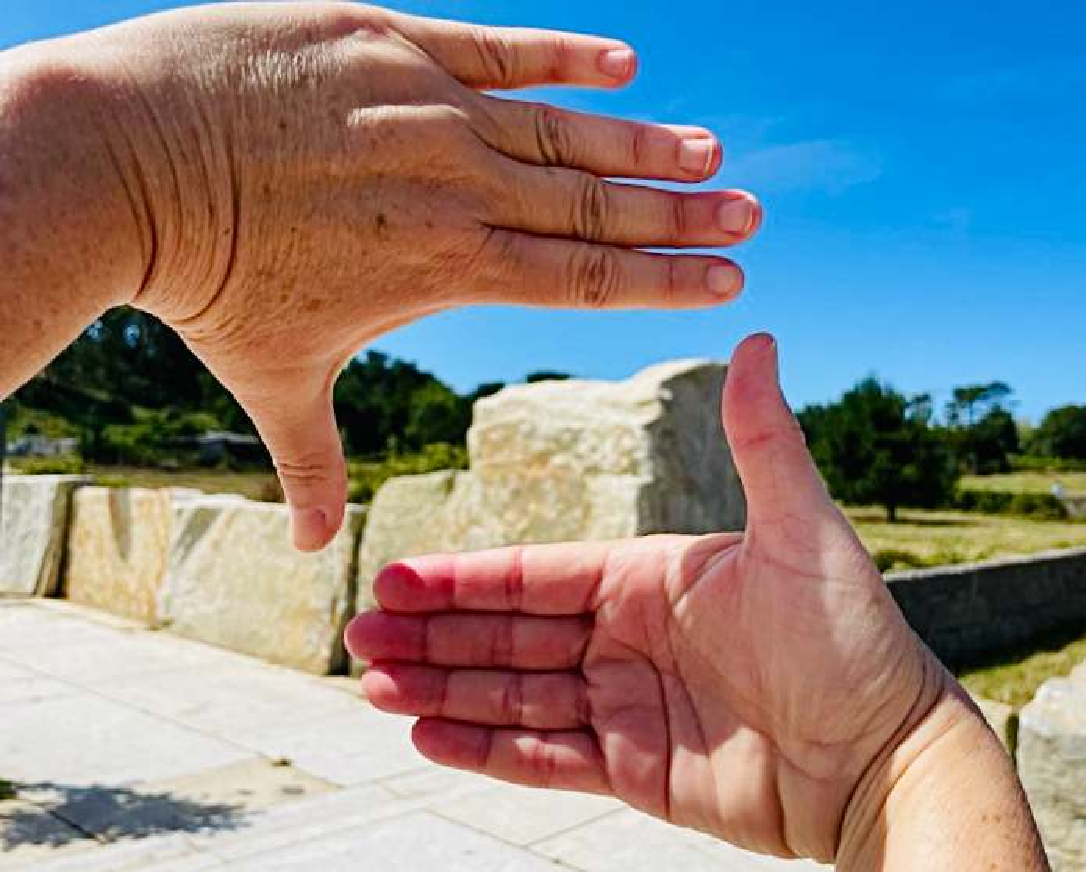
\includegraphics[width=2.76866in,height=2.22294in]{figuras/composicao-uso-maos.pdf.compressed.pdf}
	\figurenote{Foto realizada pelo autor.}
\end{figure}

Além disto, existe um plano da imagem que funciona como uma janela
imaginária na frente da câmera. Neste caso, o tamanho do plano da
imagem depende da lente e da distância da cena à câmera.

Os planos podem ser classificados quanto à distância entre a lente e o
objeto e a denominação varia um pouco de autor para autor:

Primeiro Plano ou \emph{foreground} (\emph{FG}) objetos próximos ao
espectador ou à câmera;

Plano intermediário ou \emph{midground} (PM/\emph{MG}) --- objetos um
pouco mais distantes do espectador ou câmera;

Plano de fundo ou \emph{background} (PG/\emph{BG}) --- para objetos que
estão mais distantes

\emph{Progressão visual} é um último termo classificado por
\textcite{block2021visual} que se refere conceitualmente
a uma coisa que se transforma em outra. Ao abordar a ideia de um Ponto
que se transforma em Linha e se transforma em Plano, remete à conhecida
Teoria da Forma de \emph{Kandinsky}, e a aplica a sequências narrativas
do cinema. Ele nos dá inúmeros exemplos de filmes em que a progressão de
imagens simplificadas que se tornam complexas, afetando a intensidade
visual: \textcquote[7]{block2013visual}[.]{Em \emph{The Birds}\footnotemark (1963),
	de Hitchcock, há progressões visuais à
	medida que os pássaros se reúnem e atacam. Assista à progressão visual
	na sequência do milharal em North by Northwest
	(1959)\footnotemark}%
\footnote{Referência deste filme somente na 2\textordfeminine.~edição, de 2013}%
\footnotetext{Filme \emph{\enquote{\href{https://youtu.be/sIY7BQkbIT8}{North by Northwes}}}
	em Movieclips.
}

Entretanto, nosso objetivo neste subitem não é explorar todas as
questões especificas da narrativa, mas definir os elementos visuais que
a compõem. Os 7 componentes visuais básicos, espaço, linha, forma,
tonalidade, cor, movimento e ritmo são apresentados de forma lúdica no
texto de \textcite{block2021visual}:

\begin{displaycquote}[9]{block2021visual}[.]
	O primeiro passo é pegar esse elenco de personagens, chamados de
	componentes visuais, e descobrir quem eles são. É um elenco ao qual
	estamos presos, mas é um ótimo elenco. Na verdade, esses sete membros do
	elenco são capazes de interpretar qualquer papel, qualquer humor,
	qualquer emoção, e são ótimos na televisão, na tela do computador ou na
	tela grande
\end{displaycquote}

Como se sabe, a maioria destes componentes visuais são considerados
igualmente na pintura, entretanto de forma diferente. Temos como
exemplo o componente visual \emph{movimento,} que no cinema e
audiovisual se torna aparente devido à sequência de imagens. Já na
pintura, a tela, apesar de se configurar como única, pode trazer
representações de movimentos por meio da organização das formas, dando
mobilidade ao olhar do espectador.

Para construir uma estrutura visual utilizando os componentes visuais
básicos é necessário considerar o \emph{Princípio de Afinidade e
	Contraste,} que podemos tratar como Semelhança e Diferença. Este
princípio quando aplicado aos 7 elementos visuais, determina a maior ou
a menor \emph{intensidade visual,} capaz de gerar reações emocionais
distintas junto ao público espectador. \textcquote[13]{block2021visual}[.]{Quanto maior o
	contraste em um componente visual, maior o crescimento da intensidade
	visual. Quanto maior a afinidade de um componente visual, maior a
	redução da intensidade visual}

Não pretendemos criar uma receita de bolo, até porque, em geral, o
artista não consegue se fixar muito dentro de qualquer sistema, a não
ser o dele próprio. Mas atributos como afinidade e contraste podem ser
úteis para organizar os elementos visuais e dar direcionamento a um
projeto pictórico.

A escala tonal de cinzas, muito usada na pintura, é o exemplo
apresentado por Block para demostrar o \emph{Princípio de Afinidade e
	Contraste}. O máximo de contraste é atingido com as duas pontas da
escala, ou seja, o preto e o branco.

\begin{figure}
	\caption{Contraste máximo em preto e branco.}
	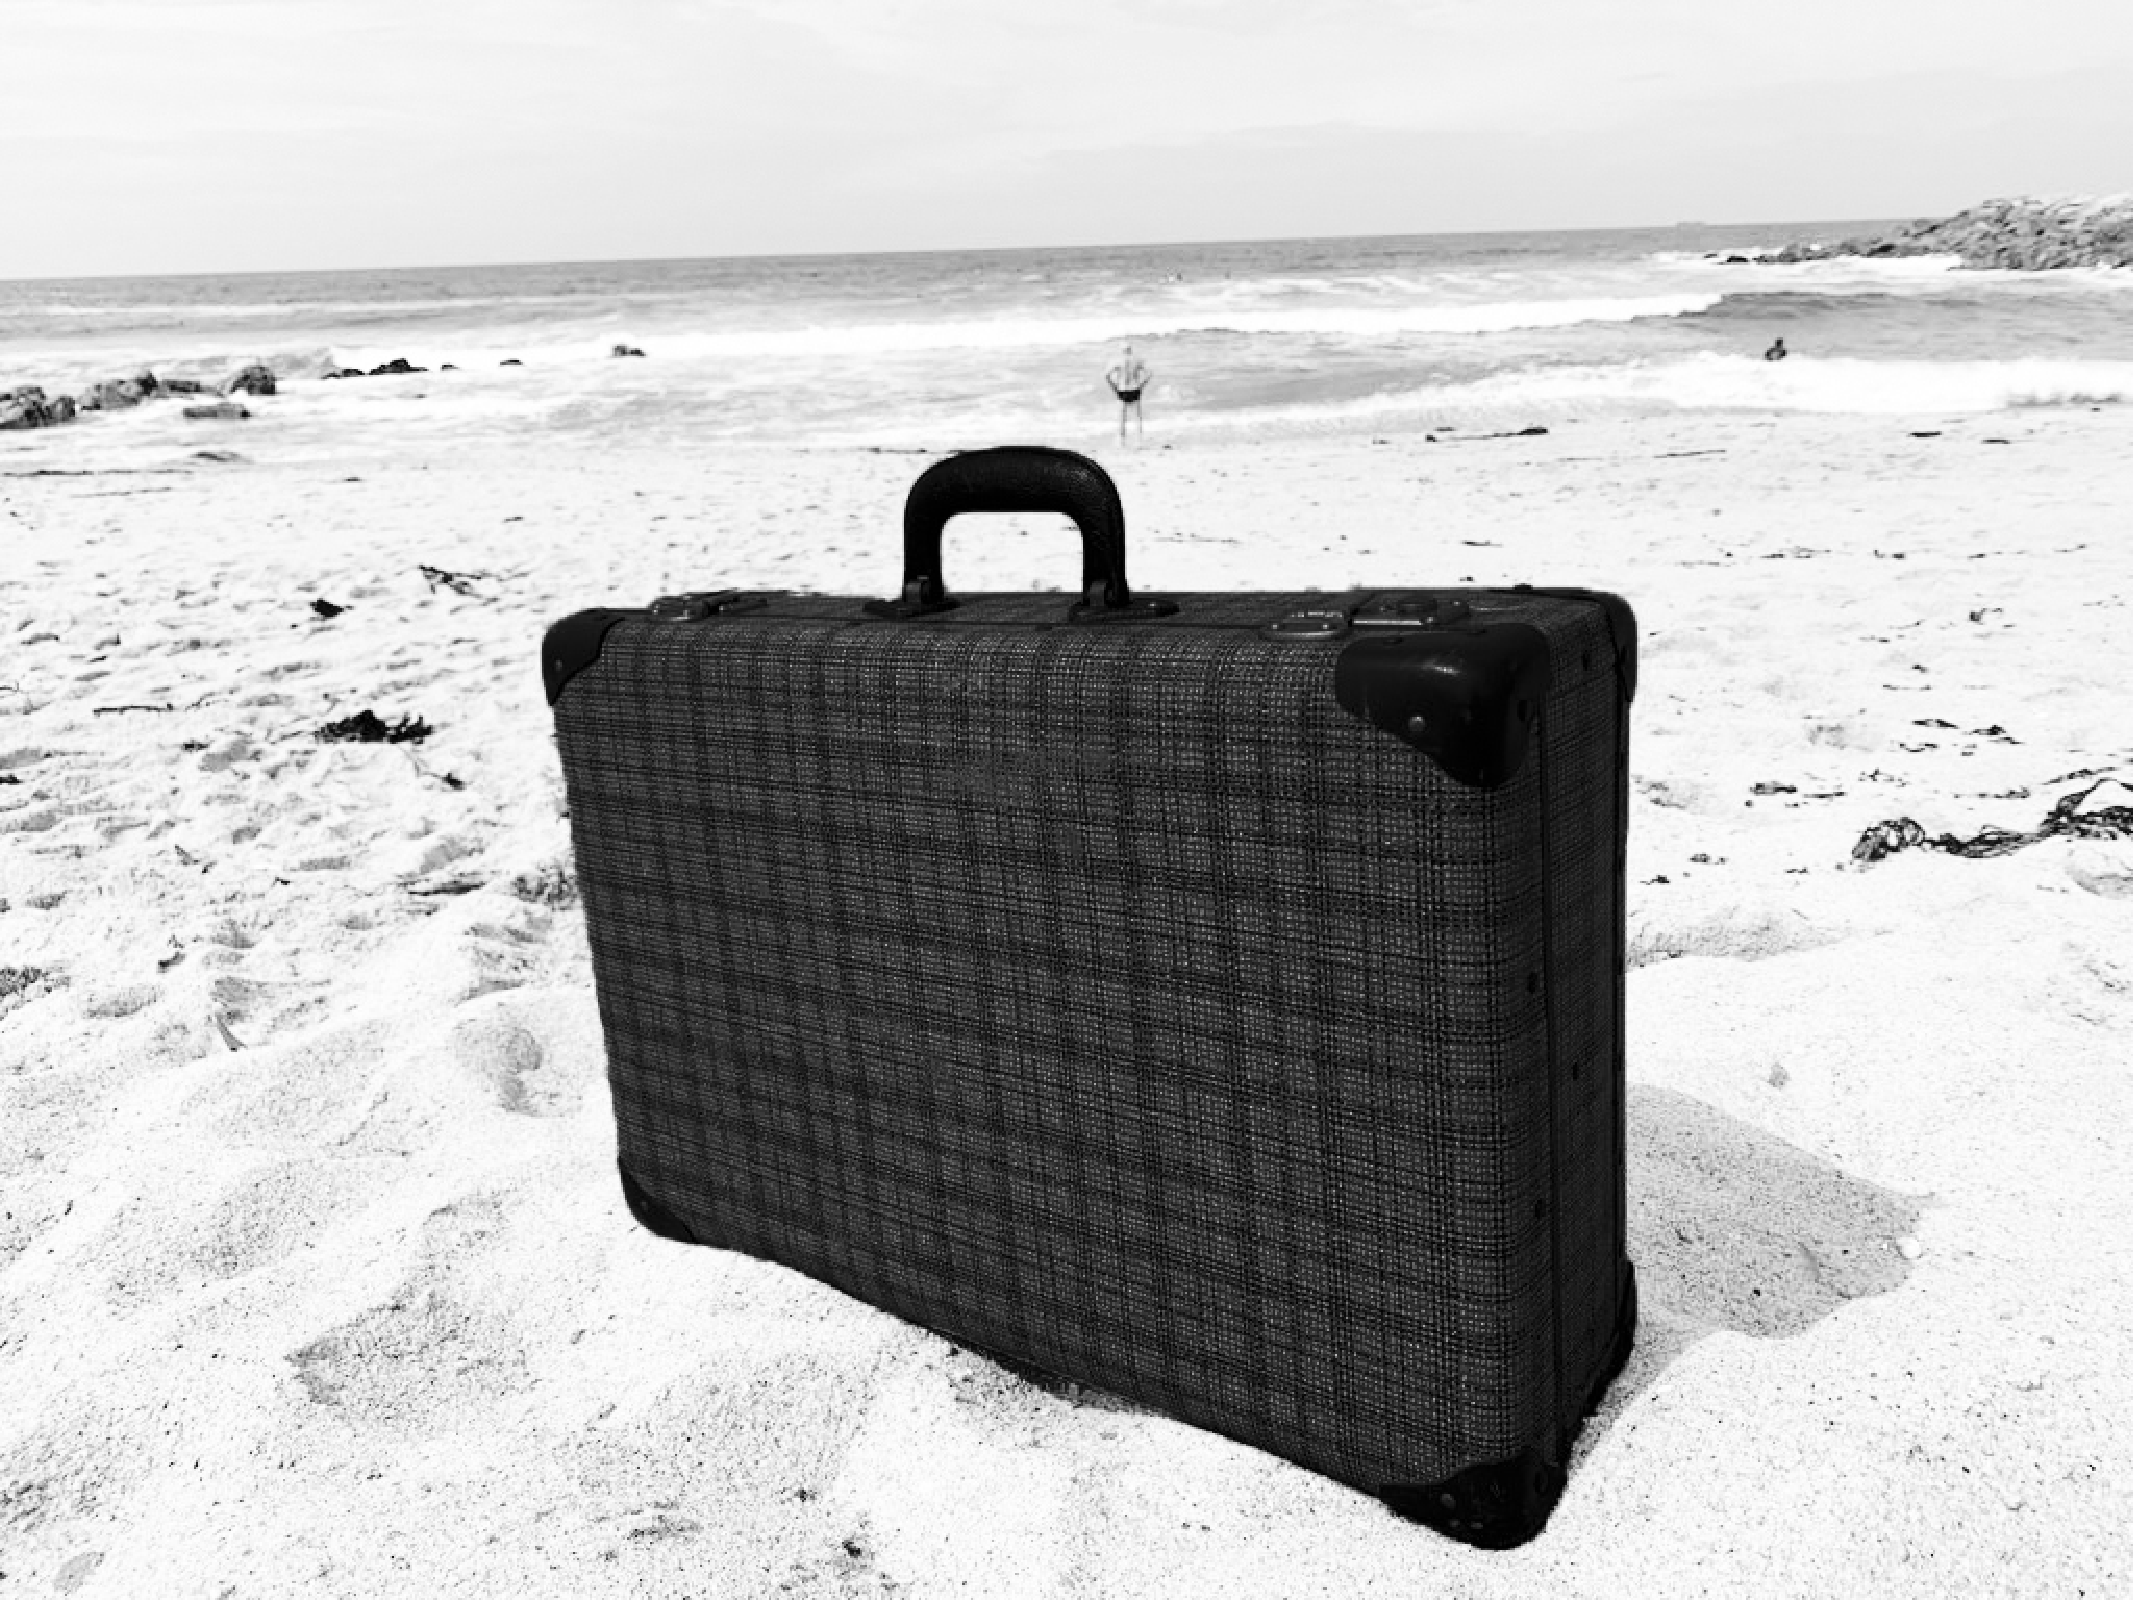
\includegraphics[width=5.90139in,height=4.42639in]{figuras/contraste-maximo-preto-branco.pdf.compressed.pdf}
	\figurenote{Foto do autor, edição de Tatyana Arruda.}
\end{figure}

Já a \emph{Afinidade} é caracterizada por grupos de tons vizinhos, como
nas imagens abaixo.

\begin{figure}
	\caption{Afinidade na escala de tons.}
	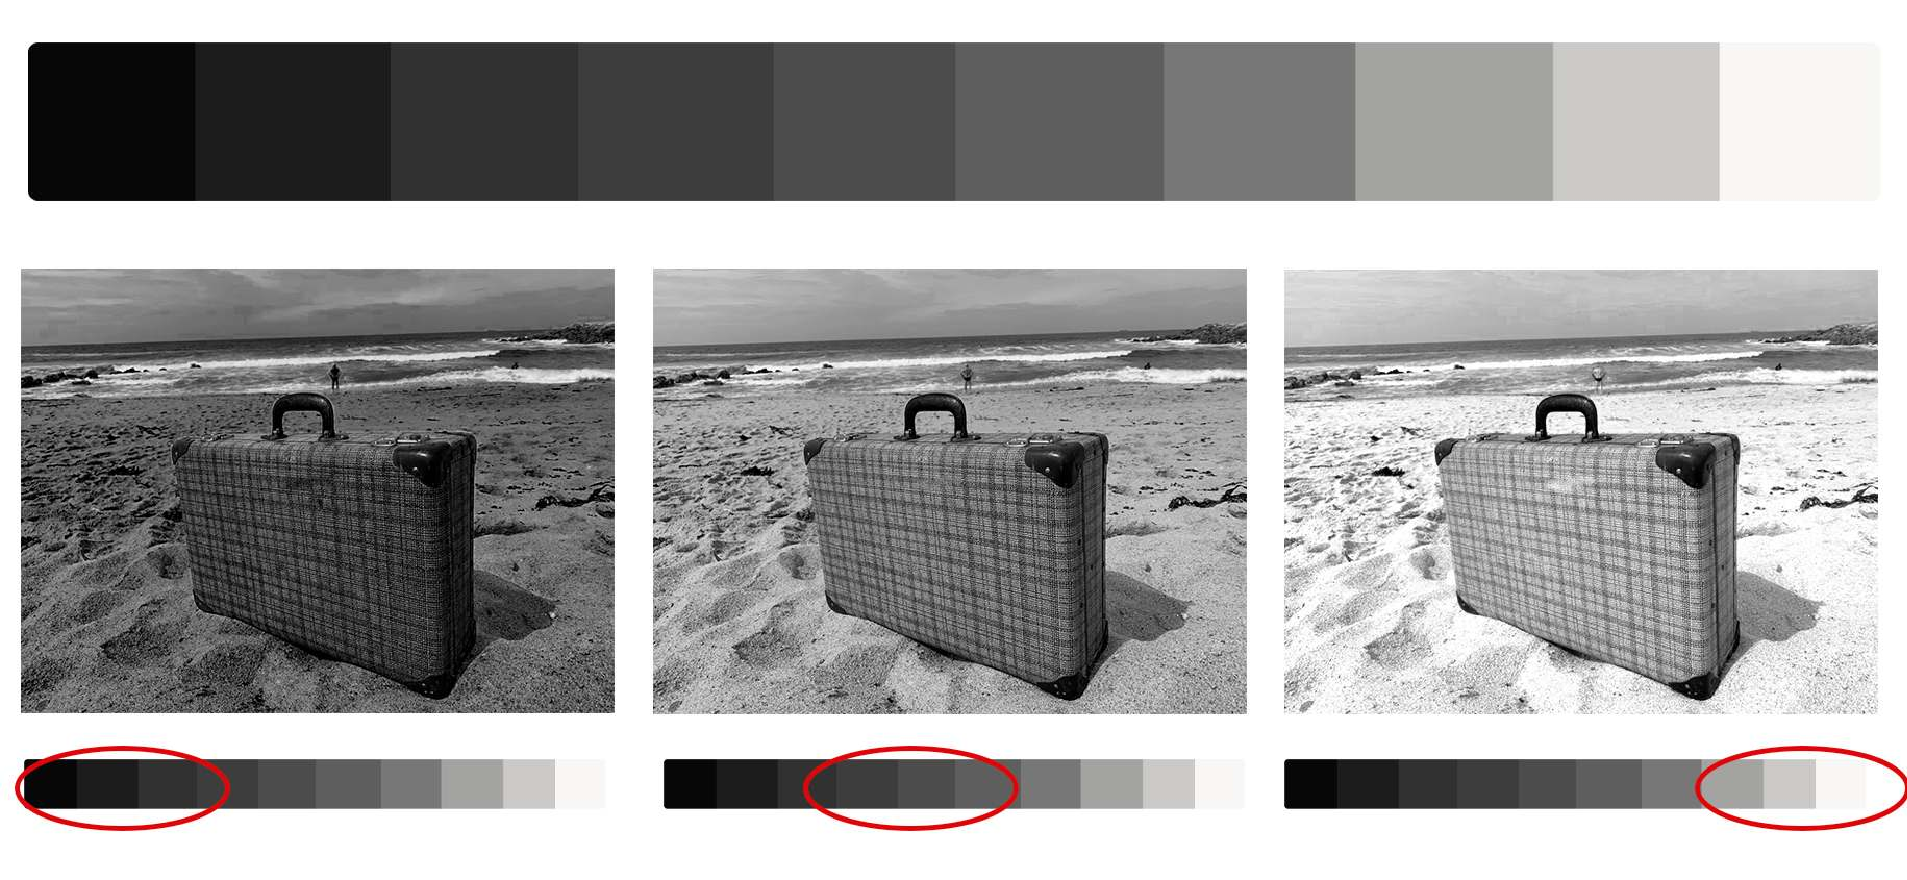
\includegraphics[width=5.40139in,height=2.72361in]{figuras/afinidade-escala-tons.pdf.compressed.pdf}
	\figurenote{Foto do autor, edição de Tatyana Arruda}
\end{figure}

O \emph{Princípio de Afinidade e Contraste} pode ser usado dentro de um
plano, de um plano para outro e de uma sequência para outra com a
finalidade de aumentar ou diminuir a dramaticidade do filme. Simples de
se compreender o \emph{Princípio da Afinidade e Contraste}, mas devido à sua
complexidade na utilização, Block nos propõe que cada um dos sete
componentes visuais básicos e seus subcomponente, façam referência ao
Princípio de Afinidade e Contraste. Assim é possível sua aplicação
prática da produção e controlar a Estrutura Visual do filme.

A estrutura da narrativa da história se vincula à estrutura visual do
filme a partir de três partes básicas: exposição (início), conflito
(meio) e resolução (desfecho). Através de gráficos, Block também
comprova que o uso da quantidade de contraste ou afinidade nos
componentes visuais mantém uma relação direta com o desenvolvimento da
intensidade do conflito da história.

O estudo da proposta de Block para construção da narrativa visual do
filme, baseado no princípio de contraste e afinidade em muito se parece
com as estratégias compositivas na pintura. São claras as aproximações
com as investigações sobre percepção em toda a história da arte, desde
os tratados renascentistas até as propostas dos teóricos da Bauhaus,
passando por Rudolf Arnheim, citado na bibliografia do texto de Block.

Na estrutura narrativa da história, é possível posicionar
estrategicamente o clímax, de acordo com os objetivos dos roteiristas,
conforme os gráficos de graus de intensidade do conflito posicionados
em uma escala que relaciona o tempo de duração do filme aos três
momentos da narrativa: exposição, conflito e resolução. A resolução é o
final da história, quando o conflito termina, \emph{diminuindo a
	intensidade} tanto da história quanto a intensidade visual, segundo o
\emph{Princípio de Afinidade e Contraste.} \parencite{block2021visual}

Com a finalidade de deixar menos cansativa a leitura deste texto,
trazemos para esta conversa apenas o primeiro dos sete elementos
visuais. Abordaremos, a seguir, o Espaço, em uma perspectiva mais
operacional e prática. O Espaço define a tela sobre a qual todos os
outros componentes visuais são vistos. São quatro as possibilidades de
escolha do espaço a serem considerados em uma \emph{locação} (espaço
real onde são realizadas as tomadas de câmera): profundo, plano,
limitado e ambíguo. O \emph{espaço profundo} se caracteriza pela ilusão
de profundidade em uma imagem bidimensional. Algumas \emph{pistas} são
criadas para convencer o observador de que aquele espaço tem
profundidade. Sabemos que esta ideia se multiplicou no período
Renascentista e durante muito tempo e até hoje é uma das bases da busca
pelo realismo na pintura. O cinema nasce com a \emph{brincadeira} de
Lumière com esta ideia, através de seu trem invadindo a sala de cinema.
O espaço profundo nas imagens bidimensionais trabalha com a sugestão
para o público de algo que não existe no mundo real, sobre uma tela
plana. É importante esclarecer que o termo espaço profundo não é um
sinônimo de profundidade de campo. Espaço profundo é a superação da
planaridade da tela. A bidimensionalidade da tela é superada de maneira
ilusória pelo que Block chama de \emph{sinais de profundidade.} O
objetivo de muitos cinematógrafos é convencer seu público de que o
espaço profundo é real, então são usados artifícios, ou pistas, que
sugerem a existência de objetos mais próximos e mais afastados. A mais
importante destas pistas é a \emph{perspectiva}. Block explica que o
espectador de um filme só percebe a perspectiva de um, dois e até no
máximo três pontos. Trabalhar a \emph{progressão visual}, se utilizando
da movimentação de vários pontos de vista é uma estratégia para
aumentar ou diminuir a ilusão de profundidade. Quanto maior a
quantidade de pontos de fuga, maior a ilusão de espaço
profundo.

\begin{figure}
	\caption{\artname{Odette Boudet}{Caminho cor de rosa}{2022}}

	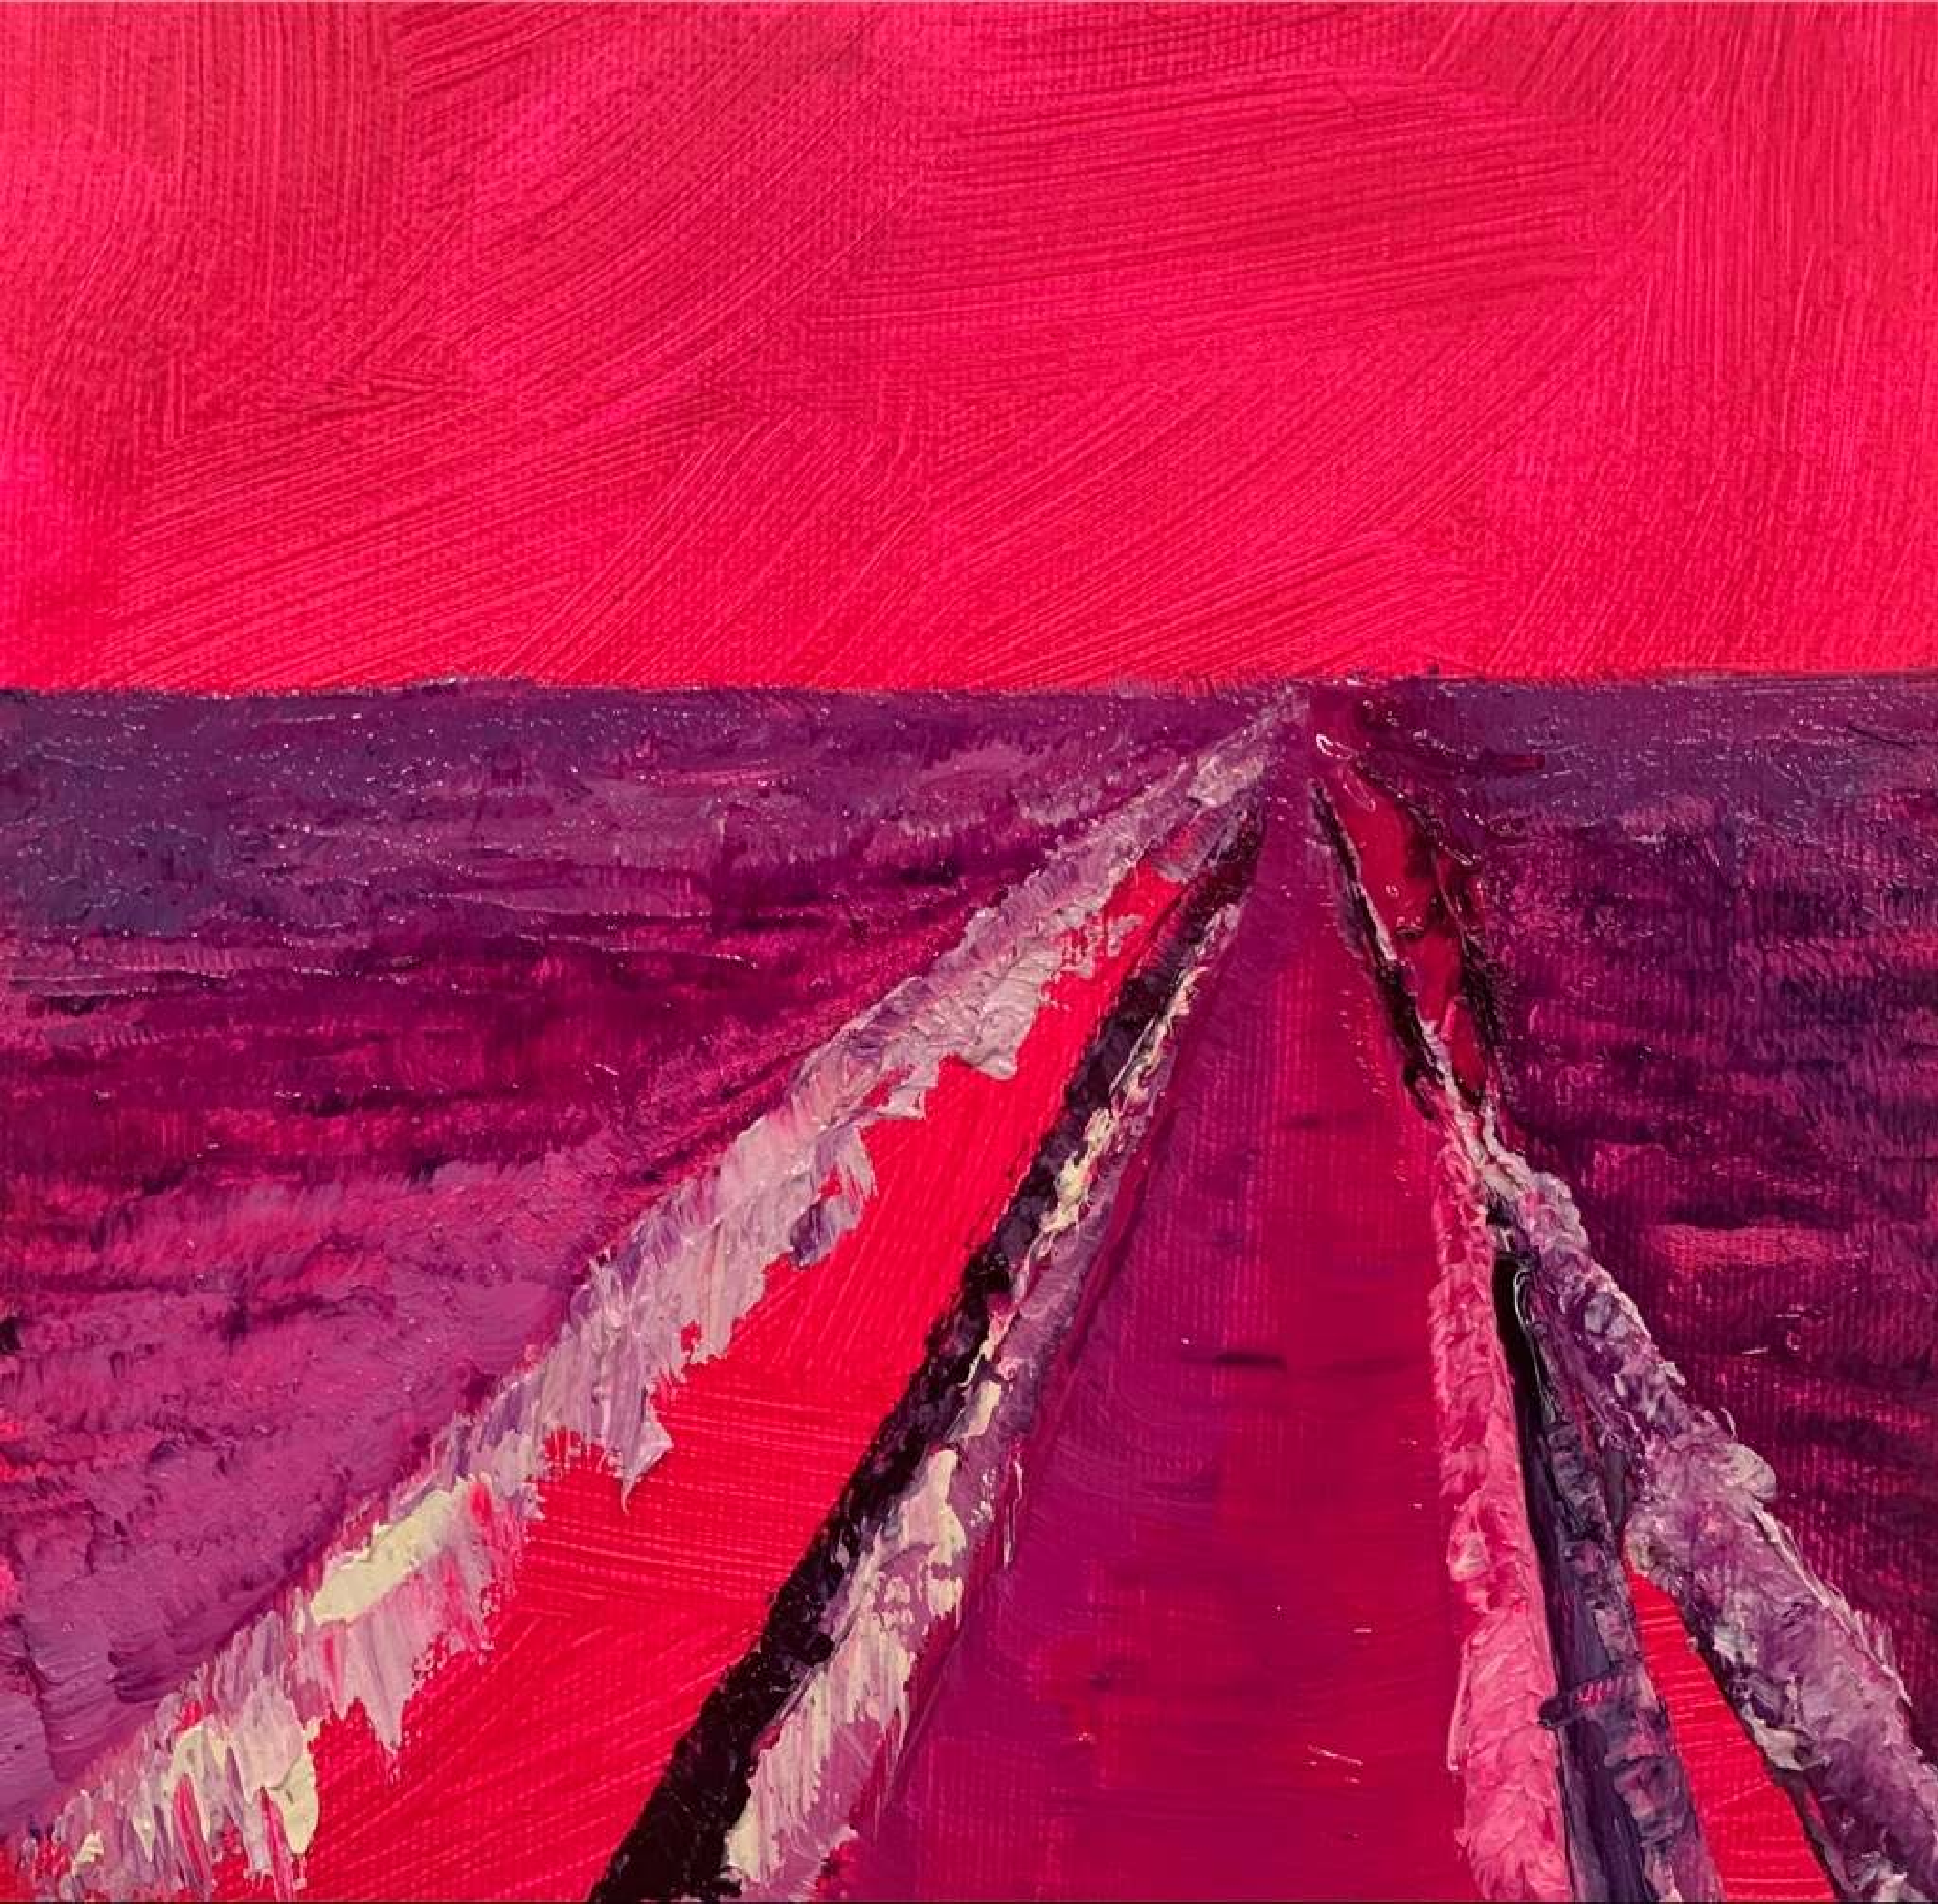
\includegraphics[width=2.07143in,height=2.03511in]{figuras/odette-caminho-cor-rosa-2022.pdf.compressed.pdf}
	\figurenote{\series{Espaço no ecrã}. \oil. \artsize{20 x 20 x 3.5}. Foto da autora.}
\end{figure}

\textcquote[24]{block2021visual}[.]{Um ponto de fuga criará a ilusão de profundidade, mas adicionar um
	segundo ou terceiro ponto aumentará a ilusão de espaço profundo} . O olho do observador
é atraído pelos pontos de fuga. Quando os pontos de fuga estão dentro da
tela atraem mais atenção do público do que quando estão fora da tela.
Observar a relação destes pontos com o posicionamento dos atores é uma
estratégia fundamental para manter a atenção do espectador.

Outras duas \emph{pistas} descritas por Block para tratar do espaço
profundo são a diferença de tamanho dos objetos ou atores e o
movimento. A organização de atores por planos próximos (FG), planos
médios e de fundo~(BG), evidenciando diferentes tamanhos, foi utilizada
em \emph{Cidadão Kane} (1941), de Orson Welles. Esta estratégia é
chamada de encenação em profundidade.

\begin{figure}
	\caption{Frame do filme Cidadão Kane com três planos em foco}
	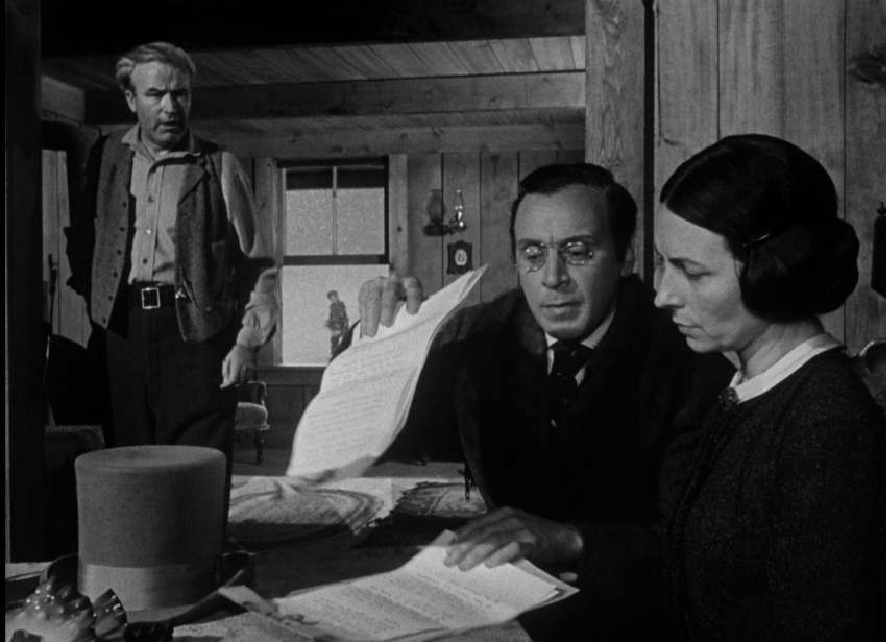
\includegraphics[width=.6\linewidth]{figuras/frame-cidadao-kane.pdf.compressed.pdf}
	\figurenote{Fonte: \hiperlink{https://outrolado.com.br/2020/12/08/a-proposito-de-cidadao-kane/}
		{Outro Lado}}
\end{figure}

Na história da pintura, a organização em planos foi muito explorada por
meio da precisão geométrica, tanto em trabalhos que primavam pelo
realismo quanto nos que exploravam a abstração.

\begin{figure}
  \flushright
  \begin{minipage}{.6\linewidth}
	\caption{\artname{Pablo Picasso}{Las meninas}{1957}}
	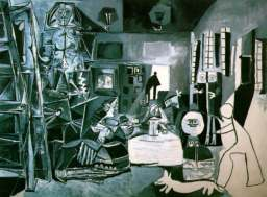
\includegraphics[width=\linewidth]{figuras/picasso-las-meninas-1957.pdf.compressed.pdf}
	\figurenote{Museo Pablo Picasso Barcelona.
		Fonte: \hiperlink{https://ca.wikipedia.org/wiki/Las\_Meninas\_\%28Picasso\%29}{Wikipedia}}
  \end{minipage}
\end{figure}

Por que será que André Bazin defendia esta estratégia? Ele se insurgia
contra as teorias do cinema dos anos 1920--1930, que preconizavam a decupagem
clássica. Acreditava na realidade objetiva~de filmes como documentários
e produções do neorrealismo italiano. Para ele, a interpretação de 
um~filme~ou cena deve ser deixada ao espectador. Tratava-se de uma posição
política contra a manipulação das imagens durante a segunda Guerra
Mundial, onde, na perspectiva fascista, o sujeito não tinha espaço para
as massas. \textcite{manevy2006}, explica:

\begin{displaycquote}[233]{manevy2006}[.]
	Bazin apontaria os efeitos da propaganda de guerra na história do cinema
	a partir de 1945 como uma espécie de divisor de águas no estatuto
	universal das imagens: tal conexão com a guerra e com a máquina da morte
	(a quem o cinema serviu, dos dois lados) representou uma espécie de
	morte do próprio cinema, uma crise de representação a que o neo-realismo
	italiano, feito nos escombros de um país derrotado, responderia como uma
	ressurreição do próprio cinema, por meio do aspecto documental
	recuperado (ninguém melhor que Bazin captaria essa dimensão)
\end{displaycquote}

Ele era partidário da ausência de montagem, substituída pelos planos
gerais (Jean Renoir), plano-sequência e profundidade de campo (Orson
Welles).

Retomando as questões da narrativa visual, além da diferença de
tamanho, outro artifício para afetar a profundidade é o movimento,
tanto de um objeto na frente da câmera quanto o movimento da própria
câmera. Encontramos um clássico exemplo disto também em \emph{Cidadão
	Kane}, que é considerado um marco histórico na utilização da
profundidade de campo com atores se movimentando diante da câmera
parada. O vídeo A técnica que fez \emph{Cidadão Kane} ser
revolucionário conta esta história\footnote{Para saber mais, André
	Bazin \enquote{A Evolução da Linguagem Cinematográfica} e David
	Bordwell: \enquote{Sobre a História do Estilo Cinematográfico}

	\url{https://www.youtube.com/watch?v=0xdN25Td_AE\&ab_channel=EntrePlanos}}.
O detalhamento das questões relativas a estes dois tipos de movimento,
dentro do plano cinematográfico, foi o que nos fez pensar em avançar com
uma proposta de projeto de pintura inspirado na estrutura visual em
questão. Ou seja, a ideia seria partir do cinema para a pintura, por
meio dos elementos considerados por \citeauthor{block2021visual}.

À medida que fomos escrevendo este capítulo, avançamos na elaboração de
um projeto pictórico, realizando esboços com a finalidade de evidenciar
aplicações dos principais conceitos relacionados ao espaço.

Conforme já mencionamos no início deste subitem, não vamos nos deter
aqui sobre os três outros subcomponentes do espaço: o espaço plano, o
espaço limitado e o espaço ambíguo. Mas temos em conta que abordar
estas categorias pode ser um método útil para se pensar formatação do
Projeto de Pintura, em desenvolvimento no ateliê, conforme veremos no
\cref{cap4-entre-projeto-processo}.

Atualmente encontramos uma tecnologia muito avançada que permite a
realização de filmes, inclusive por meio de aplicativos de celular, que
rapidamente transformam imagens estáticas em \emph{stories} de curtas e
nano filmes. Durante a realização deste trabalho, experimentamos criar
alguns pequenos filmes por meio do \emph{iMovie}\footnote{Durante esta
	investigação, também foram realizados vários experimentos em vídeo com
	o Imovie, como suporte para as reflexões sobre as relações do
	audiovisual e da pintura.} e, ao contrário do que imaginávamos,
verificamos que o processo de estruturação do espaço nestes aplicativos
ainda segue regras tradicionais de construção da imagem fílmica.

Concluímos que na teorização proposta por Block, existe um amplo espaço
para se pensar a pintura com base em termos e conceitos preconizados
pela estrutura narrativa para o audiovisual.

\section{Cenário e cor --- brincadeiras de gente grande}%
\label{sec:cenario-e-cor-brincadeiras-de-gente-grande}

Ao investigar a construção da imagem na pintura pelo olhar do cinema,
priorizando o espaço, foi preciso abordar dois outros elementos e
componentes visuais que tem uma relação fundamental com a pintura.
Surgiu então a seguinte pergunta: é possível articular o elemento cor
na criação do cenário pictórico, partindo da estrutura narrativa visual
do cinema?

Investigamos semelhanças e diferenças da utilização da cor no filme e
na pintura. Haveria uma especificidade na utilização da cor no cinema,
diferenciada daquela que vem sendo proposta pela pintura?

\paragraph{A construção do Cenário} A história do cenário é quase
tão antiga quanto a da pintura, se
manifestando na Grécia com o objetivo de adornar o teatro, passando
pela Renascença como técnica de representação na pintura em
perspectiva. Em 1660, o inglês Willian Davenant passa a representar o
ambiente de suas comédias em Londres montando cenários no palco. O
cenógrafo suíço Adolphe Appia (1862--1928), usa a luz para criar
ambientes tridimensionais a partir de sombras, propondo uma concepção
menos realista à encenação do teatro. O cenário chega ao cinema de
atrações\footnote{Filme \enquote{Le Voyage dans la lune} (1902),
	Méliès --- curta 15 minutos, 17 cenários além de telas pintadas e imagens
	em sobreposição com as mulheres estrelas.
	www.youtube.com/watch?v=UHbpgsD8zCM\&ab\_channel=TVeCinema} com painéis
imitando paisagens e criando profundidade de campo. Não havia uma
preocupação em criar ambientes realistas.

A construção de cenários arquitetônicos tridimensionais na história do
cinema, é representada por nomes italianos como \emph{Enrico Guazzoni}
e \emph{Giovanni Pastrone}. A monumentalidade dos cenários de filmes
como \emph{Brutus} (1910), \emph{Quo Vadis} (1912) e \emph{Cabíria}
(1914), influenciaram \emph{D.~W. Griffith} nas cenas de batalha do
episódio \emph{Babilônia do séc.~VI~a.c.}, em cenários de até 30 metros
edificados nos exteriores do cruzamento de Sunset e de Hollywood
Boulevard para o filme \emph{Intolerance}\footnote{Filme
	\enquote{Intolerance} (1916), \emph{D.~W. Griffith}
	www.youtube.com/watch?v=QaI3wBPIxx8} (1916).

A preocupação com o realismo, conforme vimos anteriormente, somente se
sedimentará a partir da encenação teatral de \emph{Cidadão Kane}.

Algumas concepções de cenografia se solidificaram antes mesmo da cor
surgir no cinema e ainda hoje servem de base para determinar linhas de
trabalho do diretor de arte no cinema.

\begin{description}
	\item[Realista] valorizando a materialidade do cenário, sem significados
		para além dos elementos que estão na locação.

	\item[Impressionista] O cenário é realizado a partir da atmosfera
		psicológica da ação, refletindo o drama dos personagens.\footnote{Filme
			Vento e areia, Sjöström
			\hiperlink{http://www.youtube.com/watch?v=PHipr_iPNbA\&ab_channel=magicalmediamuseum}{www.youtube.com/watch?v=PHipr\_iPNbA\&ab\_channel=magicalmediamuseum}}

	\item[Expressionista] Muitas vezes criado artificialmente, buscando
		sintonia com a atmosfera da ação. Pode ser mais teatral, sem observar
		regras de perspectiva, com construções oblíquas, com luzes e sombras
		pintadas. Ou arquitetural, como os cenários épicos do período do cinema
		italiano. Lembramos aqui a ideia de \emph{Fitzcarraldo} (1982)
		Herzog\footnote{Filme \emph{Fitzcarraldo}
			www.youtube.com/watch?v=UhB-LQ4U\_0k\&t=1898s\&ab\_channel=HernanHillkirk},
		que monta um cenário na floresta amazônica regado a ópera.
\end{description}

Um exemplo de artista contemporâneo que realiza trabalhos monumentais é
o maranhense Thiago Martins de Melo (1981), que alia à sua pintura a
escultura, instalação, além da animação \emph{stop motion.} Além disto
utiliza fisicamente, em suas obras, dispositivos de reprodução
audiovisuais, como monitores de TV e vídeo.

\begin{figure}
	\caption{\artname{Thiago Martins de Melo}{Coluna que anda sobre garras}{2016}}
	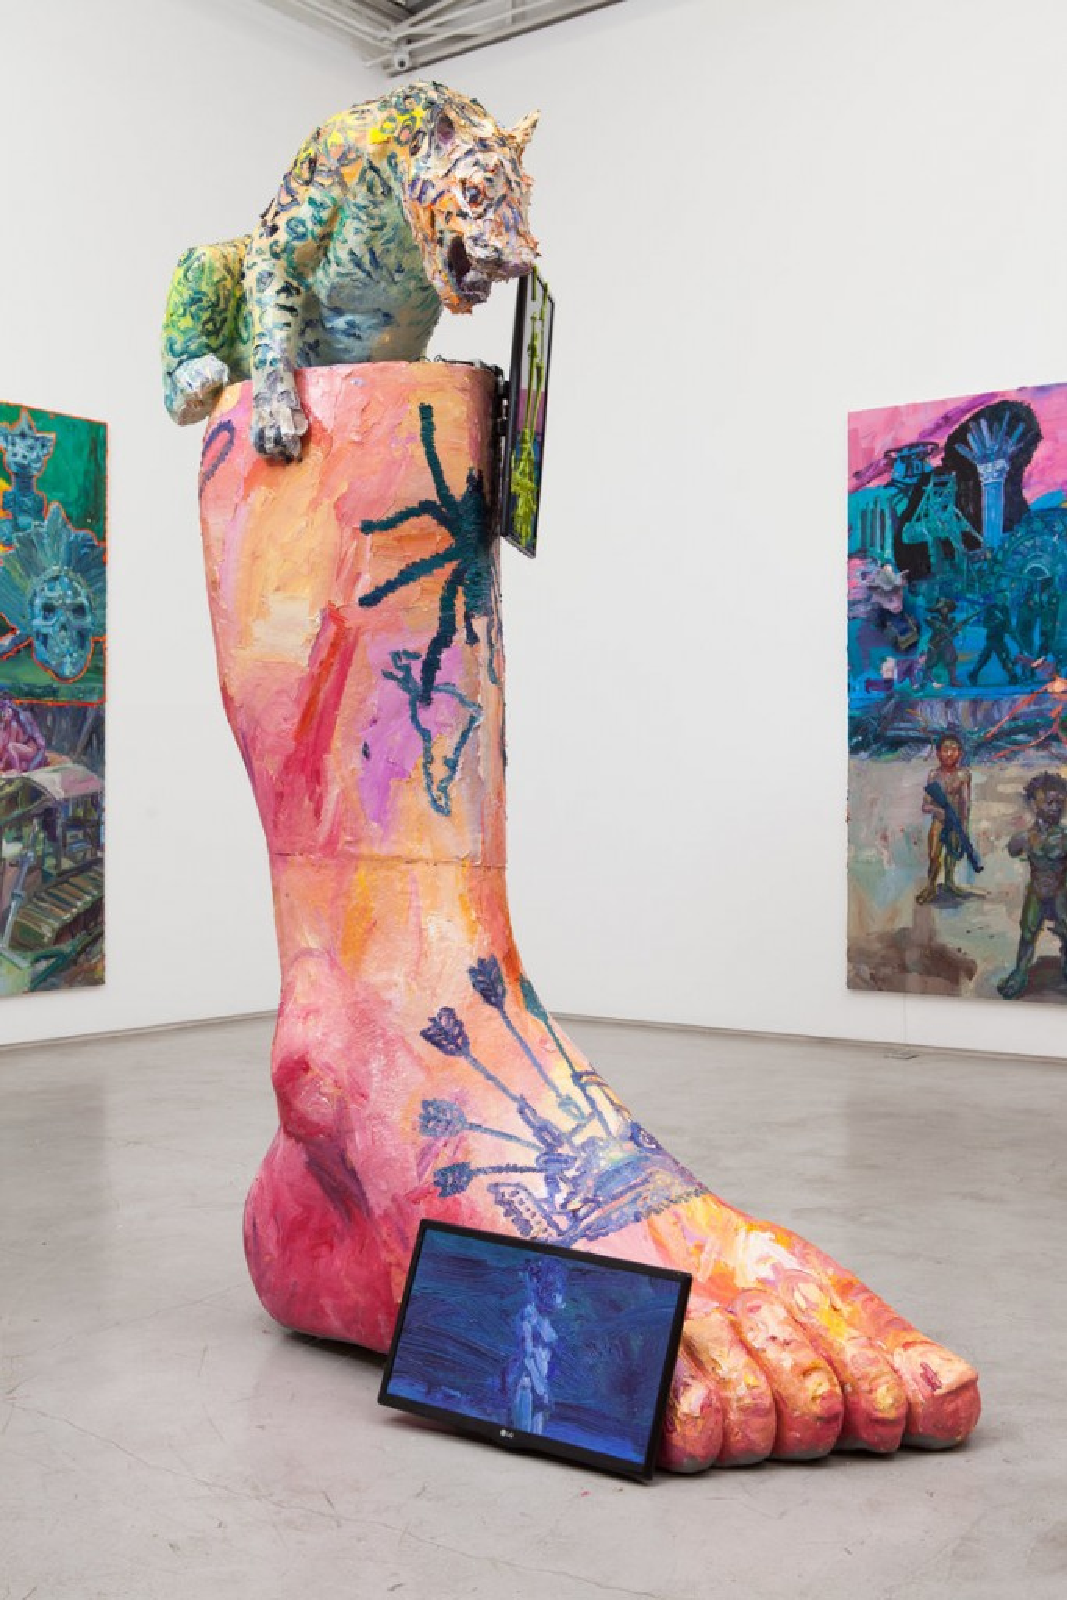
\includegraphics[width=1.32029in,height=1.97872in]{figuras/de-melo-coluna-anda-sobre-garras.pdf.compressed.pdf}
	\figurenote{Óleo sobre fibra de vidro
		resinado, poliuretano, dois monitores de TV de 22\(''\), animação stop
		motion. \artsize{245x197x70}.
		Fonte: \hiperlink{www.premiopipa.com/pag/artistas/thiago-martins-de-melo/}{Prêmio PIPA}}
\end{figure}

\paragraph{A cor} A influência da cor na estrutura cenográfica do cinema, e métodos para
estabelecer paletas na pintura, diante da evolução teórica dos estudos
da cor, são temas de grande relevância e não poderiam ficar de fora
desta dissertação. A abordagem de um assunto já tão amplamente
discutido, dentro e fora das academias de artes e de cinema, exige uma
capacidade enorme de síntese. Da mesma forma que é necessário eleger as
paletas com as quais vamos pintar um quadro ou construir um cenário
para o filme, precisamos escolher a forma como trataremos este assunto,
fundamental na construção da imagem na pintura por um olhar do cinema.
Conforme já citado acima, no quadro de componentes básicos de Block,
\enquote{a cor é um dos componentes visuais mais poderosos. A educação
	básica sobre cores geralmente é enganosa e confusa}. Abordar
cronologicamente os estudos sobre a cor, que remonta a própria história
da pintura e do cinema, seria uma possibilidade. Outra possibilidade
seria verificar como a cor é ensinada nas escolas e academias de
pintura e cinema ao longo dos anos. Decidimos retomar aqui a conversa
iniciada sobre o movimento e espaço para tratar especificamente da
aplicação da cor nas estruturas compositivas utilizadas para construir
espaços na pintura ou cenários do cinema.

Algumas das cores percebidas na natureza são parte das primeiras
palavras que os adultos ensinam às crianças. Por meio de jogos e
brincadeiras, aprendemos bem cedo os nomes das cores, nomes estes que
foram objeto de classificação teórica desde os primeiros tratados de
pintura, passando pelos contrastes de \textcite{itten1975arte} e balão cromático de
\textcite{klee1971theorie} na Escola de Arte Bauhaus e em avançados estudos
tecnológicos aplicados ao cinema. Em seus estudos sobre padrão
cromático, e das teorias de Klee, \textcite{pereira2022padrao} escreve em sua tese:

\begin{displaycquote}[60-61]{pereira2022padrao}[.]
	A forma tridimensional de um pião, ou um balão \textelp{}, serve como recurso
	para se visualizar as relações de quaisquer cores de uma paleta. Na
	superfície da forma encontram-se as gradações das cores saturadas em
	direção ao branco e a ao preto (como, por exemplo, os vermelhos na
	Figura 60). Migrando para seu interior temos as dinâmicas de saturação,
	que também podem ser mais luminosas ou escuras dependendo da altura em
	que se encontram
\end{displaycquote}

\begin{figure}
  \flushright
  \begin{minipage}{.25\linewidth}
	\caption{\artname{Marcelo Duprat}{Pião de cor com ritmo tonal de vermelhos}{2020}}
	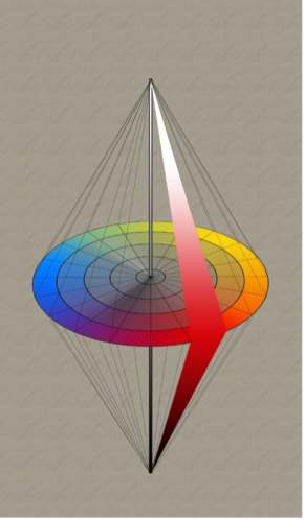
\includegraphics[width=\linewidth]{figuras/duprat-piao-cor-ritmo-tonal-vermelhos-2020.pdf.compressed.pdf}

	\figurenote{Ilustração digital. Fonte: tese doutoramento de \textcite[61]{pereira2022padrao}}
\end{minipage}
\end{figure}

Colorir casinhas e cenários são as primeiras brincadeiras lúdicas
oferecidas às crianças. Deste momento até a compreensão de tantos
estudos relacionados à cor, muito se perde da inocência e do modo
instintivo de se lidar com ela, mas o êxtase provocado por este
elemento mágico usado nos cenários de filmes de \emph{Méliès} permanece
até hoje, nos mais avançados projetos de \emph{NFT's}\footnote{NFT ---
	Non-Fungible Tokens ou \enquote{tokens não fungíveis} são ativos
	digitais certificados de forma única através de criptografias.}.

Antes do surgimento da cor no cinema, os diretores não se preocupavam
em estruturar esquemas de cor para seus filmes. Tão logo foi iniciada a
produção de filmes coloridos, a cinematografia passa a se utilizar de
esquemas de paletas para contribuir com a narrativa do filme. Desta
forma as teorias das cores já usadas na pintura serviram de instrumento
para a direção de arte compor cenários, figurinos, determinar períodos
e até mesmo criar uma atmosfera geral específica para cada roteiro.

No cenário proposto pela direção de arte, a história a ser contada quer
se colocar em um espaço que busca simular uma realidade ou uma ficção.
A articulação entre o trabalho do diretor de fotografia e o do diretor
de arte vai se materializar no \emph{set} de filmagem ao som clássico
das palavras luz, câmera~e ação, seguidas do bater da \emph{claquete},
quando a realização da captação acontece. Só depois desta etapa é que o
filme irá parar nas mãos do montador na fase de pós-produção, onde
também existe a presença do colorista que fará o tratamento de cor
usando softwares de correção da cor.

As experiências e testes do pintor na paleta para definir o caminho
cromático que será utilizado, se equivalem ao projeto visual feito pela
direção de arte ou \emph{production designer} do filme. A correção~de
cor, no cinema contemporâneo, é feita na pós-produção, com a
possibilidade da presença do diretor de~arte ou do \emph{production
	designer.} Então temos os testes de luz e a correção de cor do cinema
também.

Assim como na Escola de Arte Bauhaus, as descobertas científicas
relativas à cor foram determinantes para as mudanças no rumo estético e
conceitual, o cinema se vale da tecnologia para aprimorar as intenções
narrativas relacionadas tanto ao uso da iluminação quanto da cor. O
filme \emph{Iluminados} (2007), de Cristina Leal, nos dá um exemplo
disto, ao propor que fotógrafos de cinema utilizem o mesmo
argumento/roteiro para contar uma história a partir de seus pontos de
vista de fotografia e de iluminação \parencite{leal2008iluminados}.

\begin{figure}
	\caption{El Greco-El Expolio, 1577--1579 --- Catedral de Toledo}
	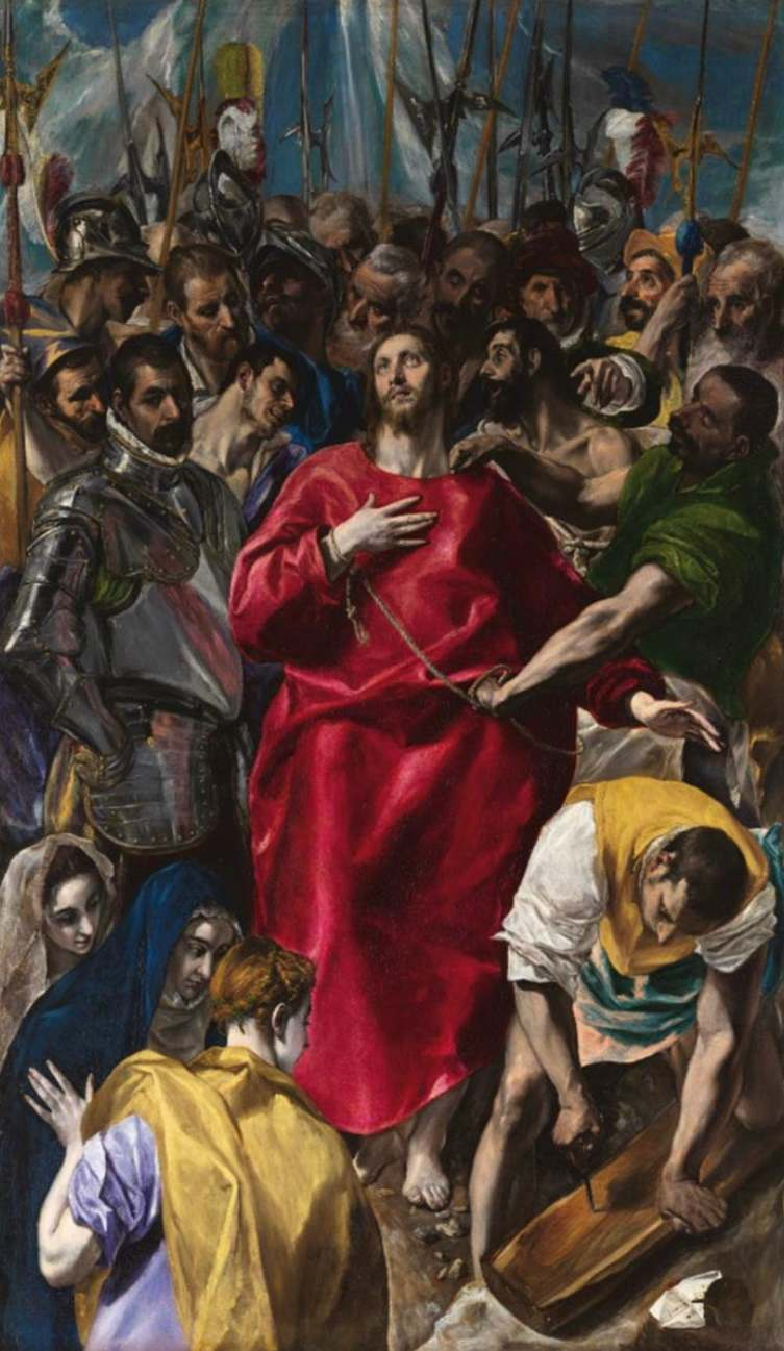
\includegraphics[width=1.96377in,height=3.38261in]{figuras/greco-el-explio.pdf.compressed.pdf}
	\figurenote{Fonte: \hiperlink{www.wikiart.org/pt/el-greco/el-expolio-1579}{Wikiart}}
\end{figure}

Se o diretor de fotografia no cinema trabalha extremamente ligado aos
movimentos de câmera, e dos vetores que conduzem o olhar do expectador,
o diretor de arte foca seu trabalho nos elementos de composição visual
(figura, cenário e objeto) para organizar o espaço que está sendo
filmado. Suas estratégias são direcionadas para o espaço viabilizado
pela câmera. A composição do cenário por meio da cor teria neste caso
uma ligação muito maior com a cor pigmento do que com a cor luz, porque
cenário e figurino têm existência material. Mas a cor luz também
precisa ser pensada, e geralmente esta tarefa é atribuída ao diretor de
fotografia. Consequentemente, poderíamos dizer que as estratégias de
direcionamento do olhar por meio da cor, que os pintores se utilizaram
ao longo da história da arte, têm uma relação maior com a função do
diretor de arte do que com a do diretor de fotografia. Se o movimento
vetorial dos olhares dos personagens, o campo/contracampo nasce do
ponto de vista ditado pela câmera, podemos considerar que a busca pela
ambientação e atmosfera do filme tem uma afinidade grande com as
escolhas que a direção de arte faz para o cenário e figurino. E isto é
fortemente interligado com todo o estudo da cor herdado da pintura.


Embora nosso foco seja a estruturação do espaço, foi necessário tratar
do problema das referências para pensar um ou mais projetos
construtivos, dentro de tantas possibilidades. No próximo capítulo,
veremos como as artistas Lucia Laguna (colagem) e Cristina Canale
solucionam esta questão na evolução de seus projetos, e como recorrem a
referências externas de outros pintores e pessoais.
